\chapter{Experimental}
\label{experimental}
This chapter will show the complete developement process of the Electronic Leadscrew based on the V-Modell. 


\section{Requirements and Logical Architecture}

In this section the developement process in the first part of the V-Modell will be described. As shown in figure \ref{V Model Requirements} this part is split into two. The requirements describe the fundamental properties of the system in order to function.
The system Logical Architecture describes how the different system components are supposed to interact with each other.

\begin{figure}
    \begin{center}
    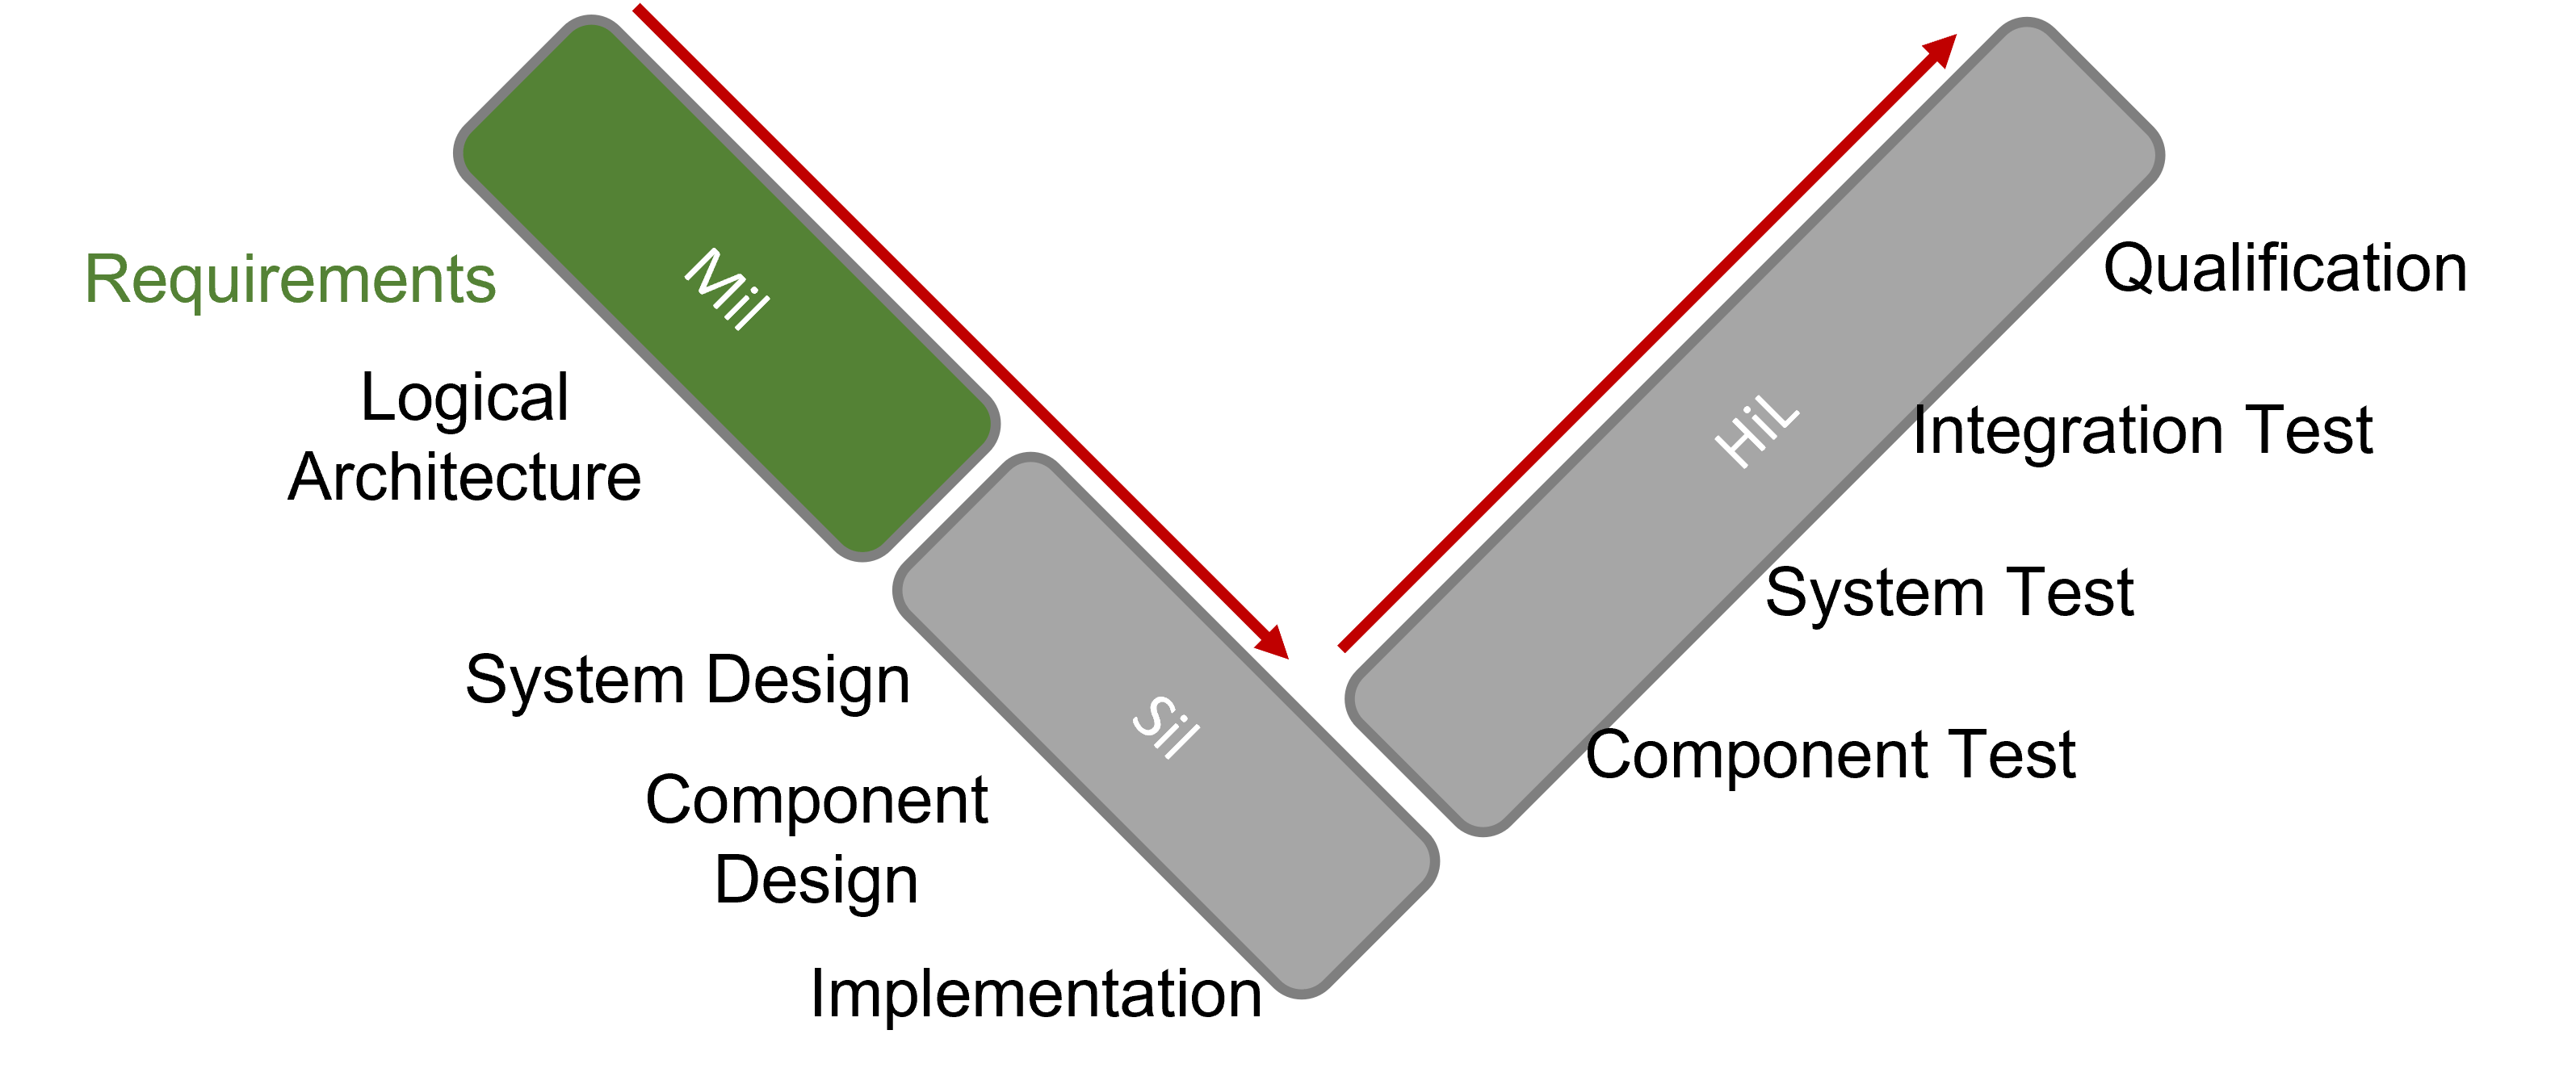
\includegraphics[width=12cm]{Pictures/V Model Requirements.png}
    \caption[V Model Requirements]{V Model Requirements Stage; Green - Developement status}
    \label{V Model Requirements}
    \end{center}
\end{figure}


\subsection{Requirements}
The developement of the System requirements was the first step in the developement process. This first step is one of the most important steps in the developement process, because it defines the functions and properties of all Systemcomponents.A selectoin of the requirements for the Human Machine Interface (HMI), the micro controller ($\mu$C), the motor and the motor controller are shown in Table \ref{Tab Key Requirements}. The full list of requirements can be found in Appendix \ref{AppendixRequirements}.

\begin{table}
    \centering
     \begin{tabular}{||c|c|c|c|c||} 
        \hline
        Req. Nr. & HMI & $\mu$C & Motor & Motor Controller \\ [0.5ex] 
        \hline\hline
        1 & Touch       & Real Time         &  Max. Torqe   & Closed Loop   \\ 
        2 & Modular     & Matlab Code Gen.  &  Min. Torqe   & Supply Voltage\\
        3 & UART Com.   & UART Com.         &  Max. Speed   & Programmable  \\
        4 & Separat PS  & Quad. Encoder     &  Min. Speed   & Resolution    \\
        5 & Mount       & GPIO              &  Space Claim  & Communication \\ [1ex] 
        \hline
     \end{tabular}
     \caption{Selection of Key Requirements for the ELS}
     \label{Tab Key Requirements}
\end{table}




\subsection{Logical Architecture}

The next step in the developement process of the ELS was to create the Logical Architecture of the System. This was done as a Toplevel Blockdiagramm as shown in Figure \ref{Logical Architecture}.

\begin{figure}
    \begin{center}
    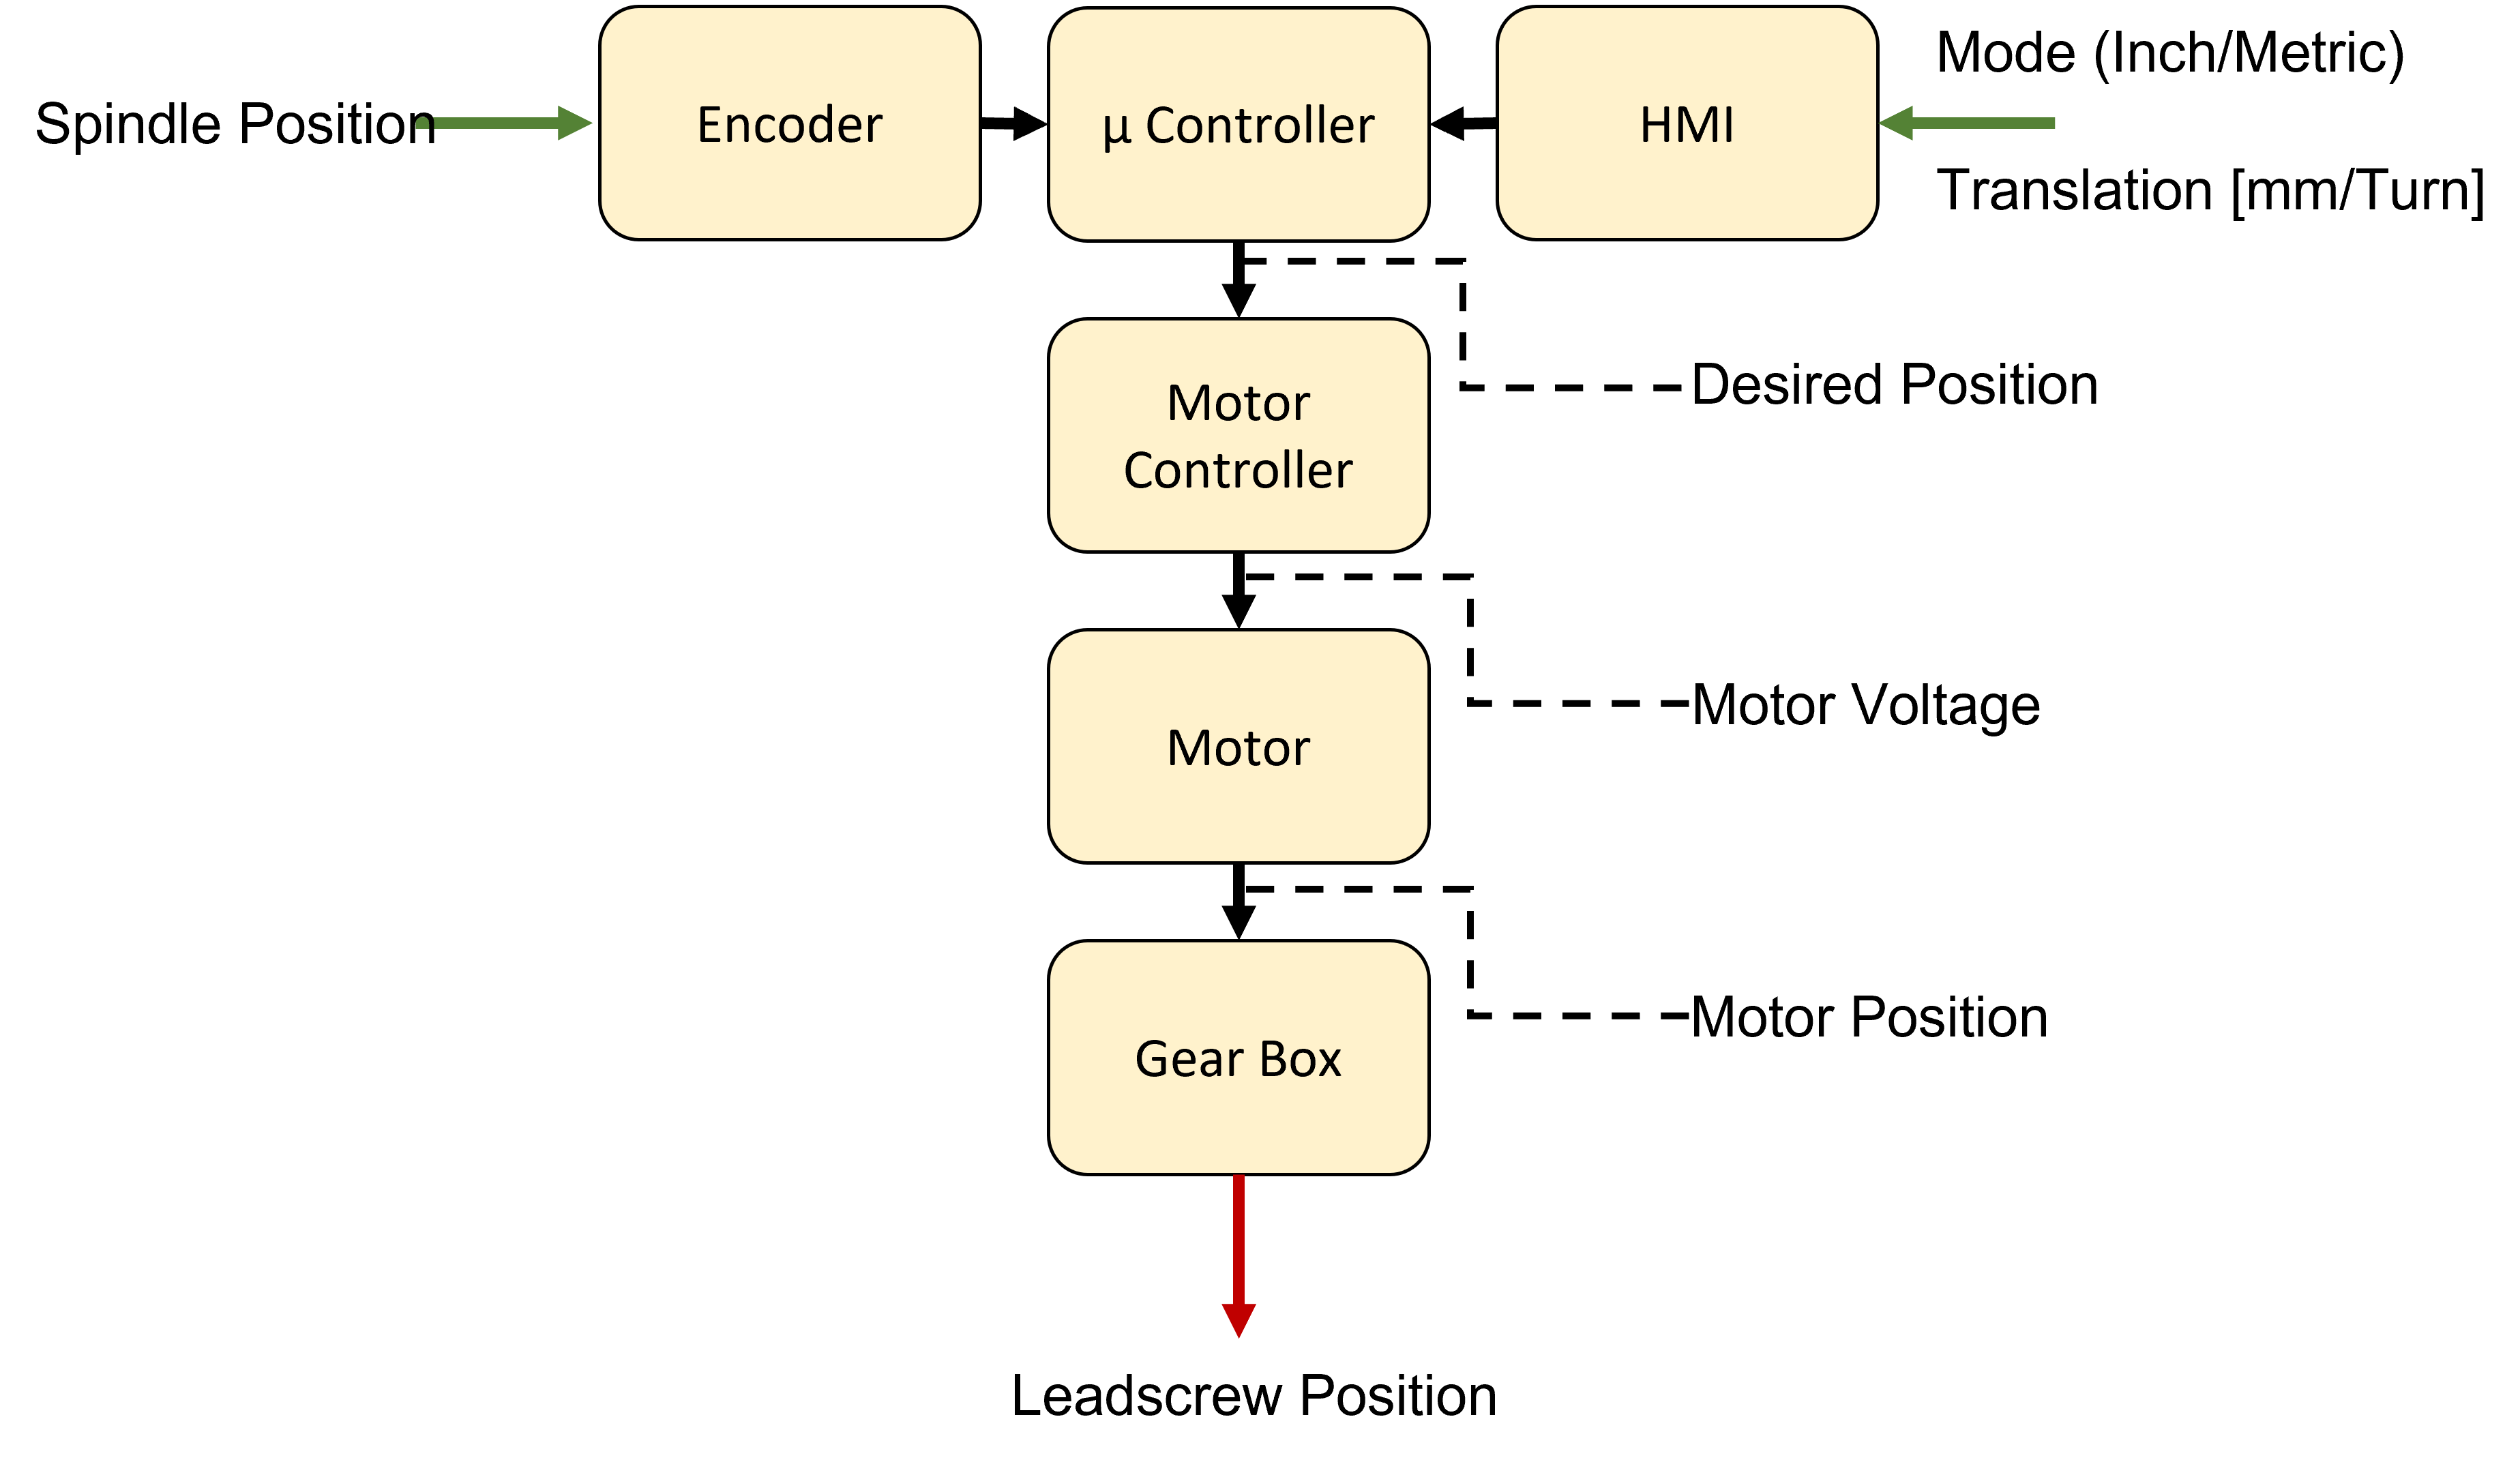
\includegraphics[width=12cm]{Pictures/Logical Architecture.png}
    \caption[Logical Architecture]{Logical Architecture}
    \label{Logical Architecture}
    \end{center}
\end{figure}

\section{System Design and Implementation}
This section describes the second half of the developement process, divided into system and component design as well as the integration of the components. This is the most time consuming process of the developement.For the system and component design, every function of each system and subsystem must be specified in detail. During the implementation phase, these functions are than transferred into the real system.\\
This developement stage is represented by the Software in the Loop (SIL) stage and is shown in Figure \ref{V Model System Design}.

\begin{figure}
    \begin{center}
    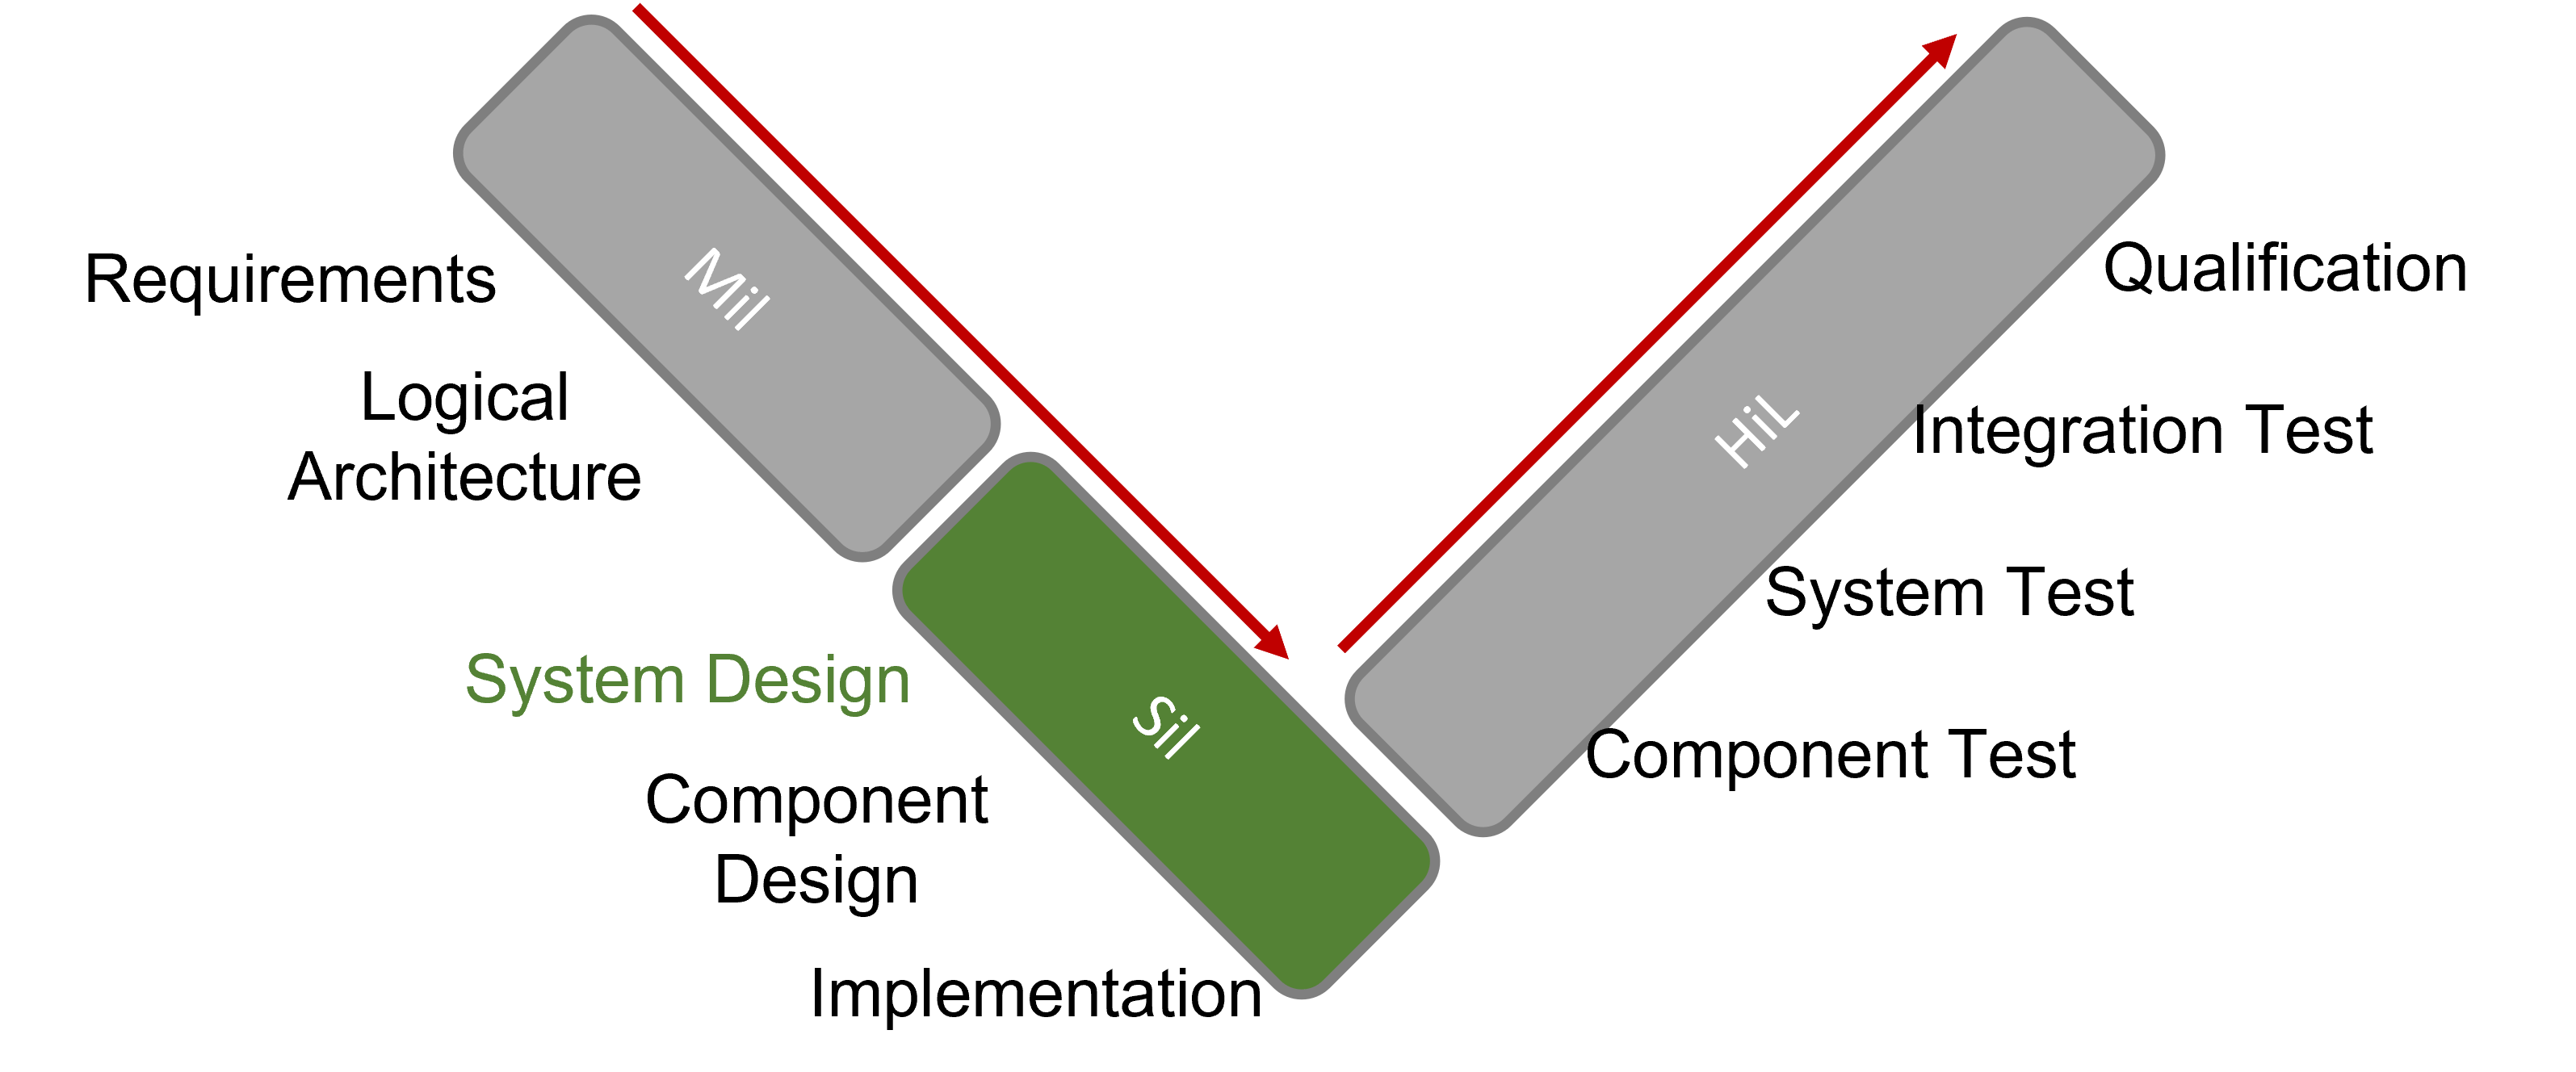
\includegraphics[width=12cm]{Pictures/V Model System Design.png}
    \caption[V Model System Design]{V Model SIL Stage; green - Developement steps SIL stage}
    \label{V Model System Design}
    \end{center}
\end{figure}

\subsection{System Design}
%%TODO: add Picture security pin
%%TODO: add Picture System design

The system design design is executed based on the previously developed system requirements and its logical architecture. The system design was approached by filling the requirements list as well as the block diagram of the logical architecture with component specific parameters. These parameters either need to be defined or found during the system design process.\\
A good example for this process is the required torque of the Leadscrew servo during a cutting process. This parameter can be found by measuring the power consumption of the AC motor for different cutting parameters with the old Leadscrew drive train. However while disassembling the original Leadscrew drive train in order to find a good place to mount the servo motor, an easier way to determine the required motor torque was found. In order to protect the Leadscrew the manufacturer secured the gear, that is driving the leadscrew with a brass pin. According to the manufacturer, this pin will shear off when more than 1.2Nm is acting on the leadscrew.\\
After this, all other parameter were determined in a similar matter. The resulting logical structure is shown in Figure \ref{System design}.

\begin{figure}
    \begin{center}
    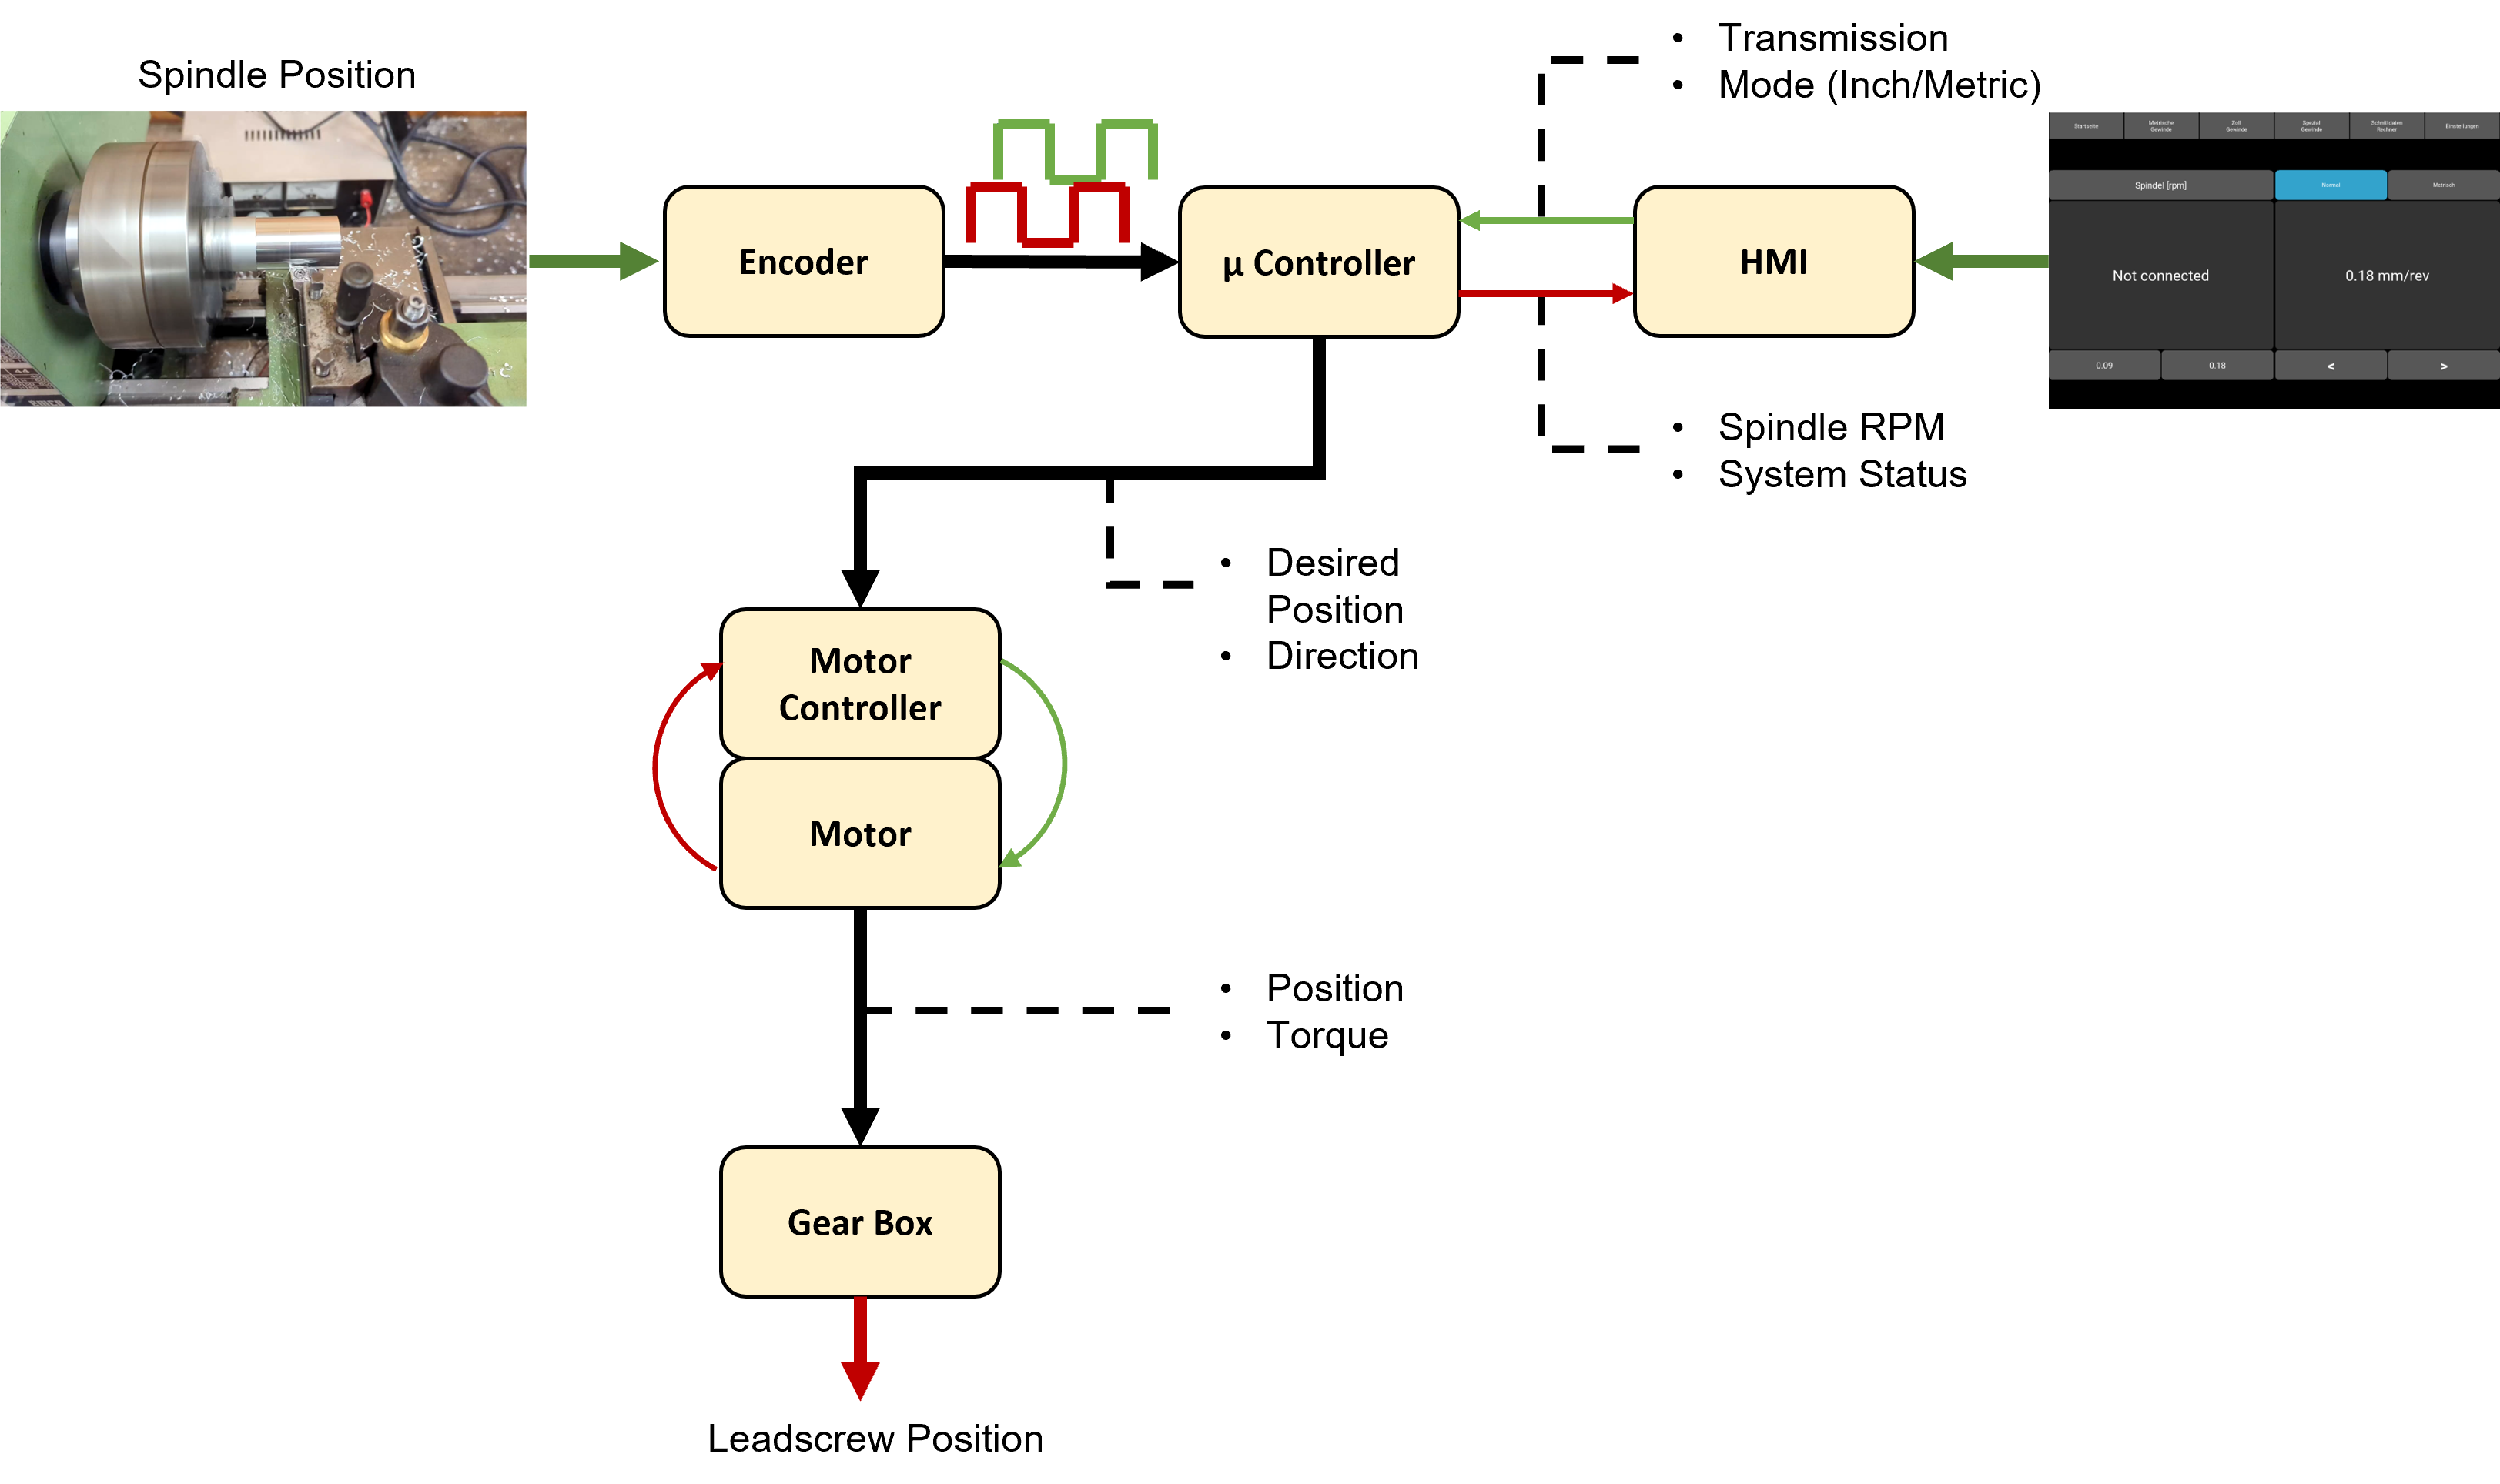
\includegraphics[width=12cm]{Pictures/SystemDesign.png}
    \caption[Block diagram of the system design]{Block diagram of the system design}
    \label{System design}
    \end{center}
\end{figure}


\subsection{Component Design}
During the component design phase, the function of each component is developed based on the previous developement steps. However the components are not jet put together as a system.

\subsubsection{HMI}
Because the HMI was required to be as modular as possible a Raspberry Pi 4 was chosen as the main component. It was combined with a 7" capacitive Touchscreen that can be bought as an accessory for the Raspberry Pi.\\
The software for the HMI was developed a main screen that shows the current RPM of the main spindle as well as the currently selected feed. Further, the main screen incorporates buttons to change the current feed rate ore mode. The mode dictates how the ELS is working. Three options are available: 

\begin{itemize}
    \item \textbf{Normal Mode} Mode for normal turning. The feed rate (mm/revolution) is selectable in 0.01 mm/rev increments.
    \item \textbf{Metric Mode} Mode for metric thread cutting. The step buttons allow to step through a list of predefined thread pitches.
    \item \textbf{Imperial Mode} Mode for imperial thread cutting. The step buttons allow to step through a list of predefined thread pitches (threads/inch).
\end{itemize}

Further, the HMI offers submenus for all available thread pitches and various other functions. The main screen of the HMI is shown in Figure \ref{HMI main Screen}.

\begin{figure}
    \begin{center}
    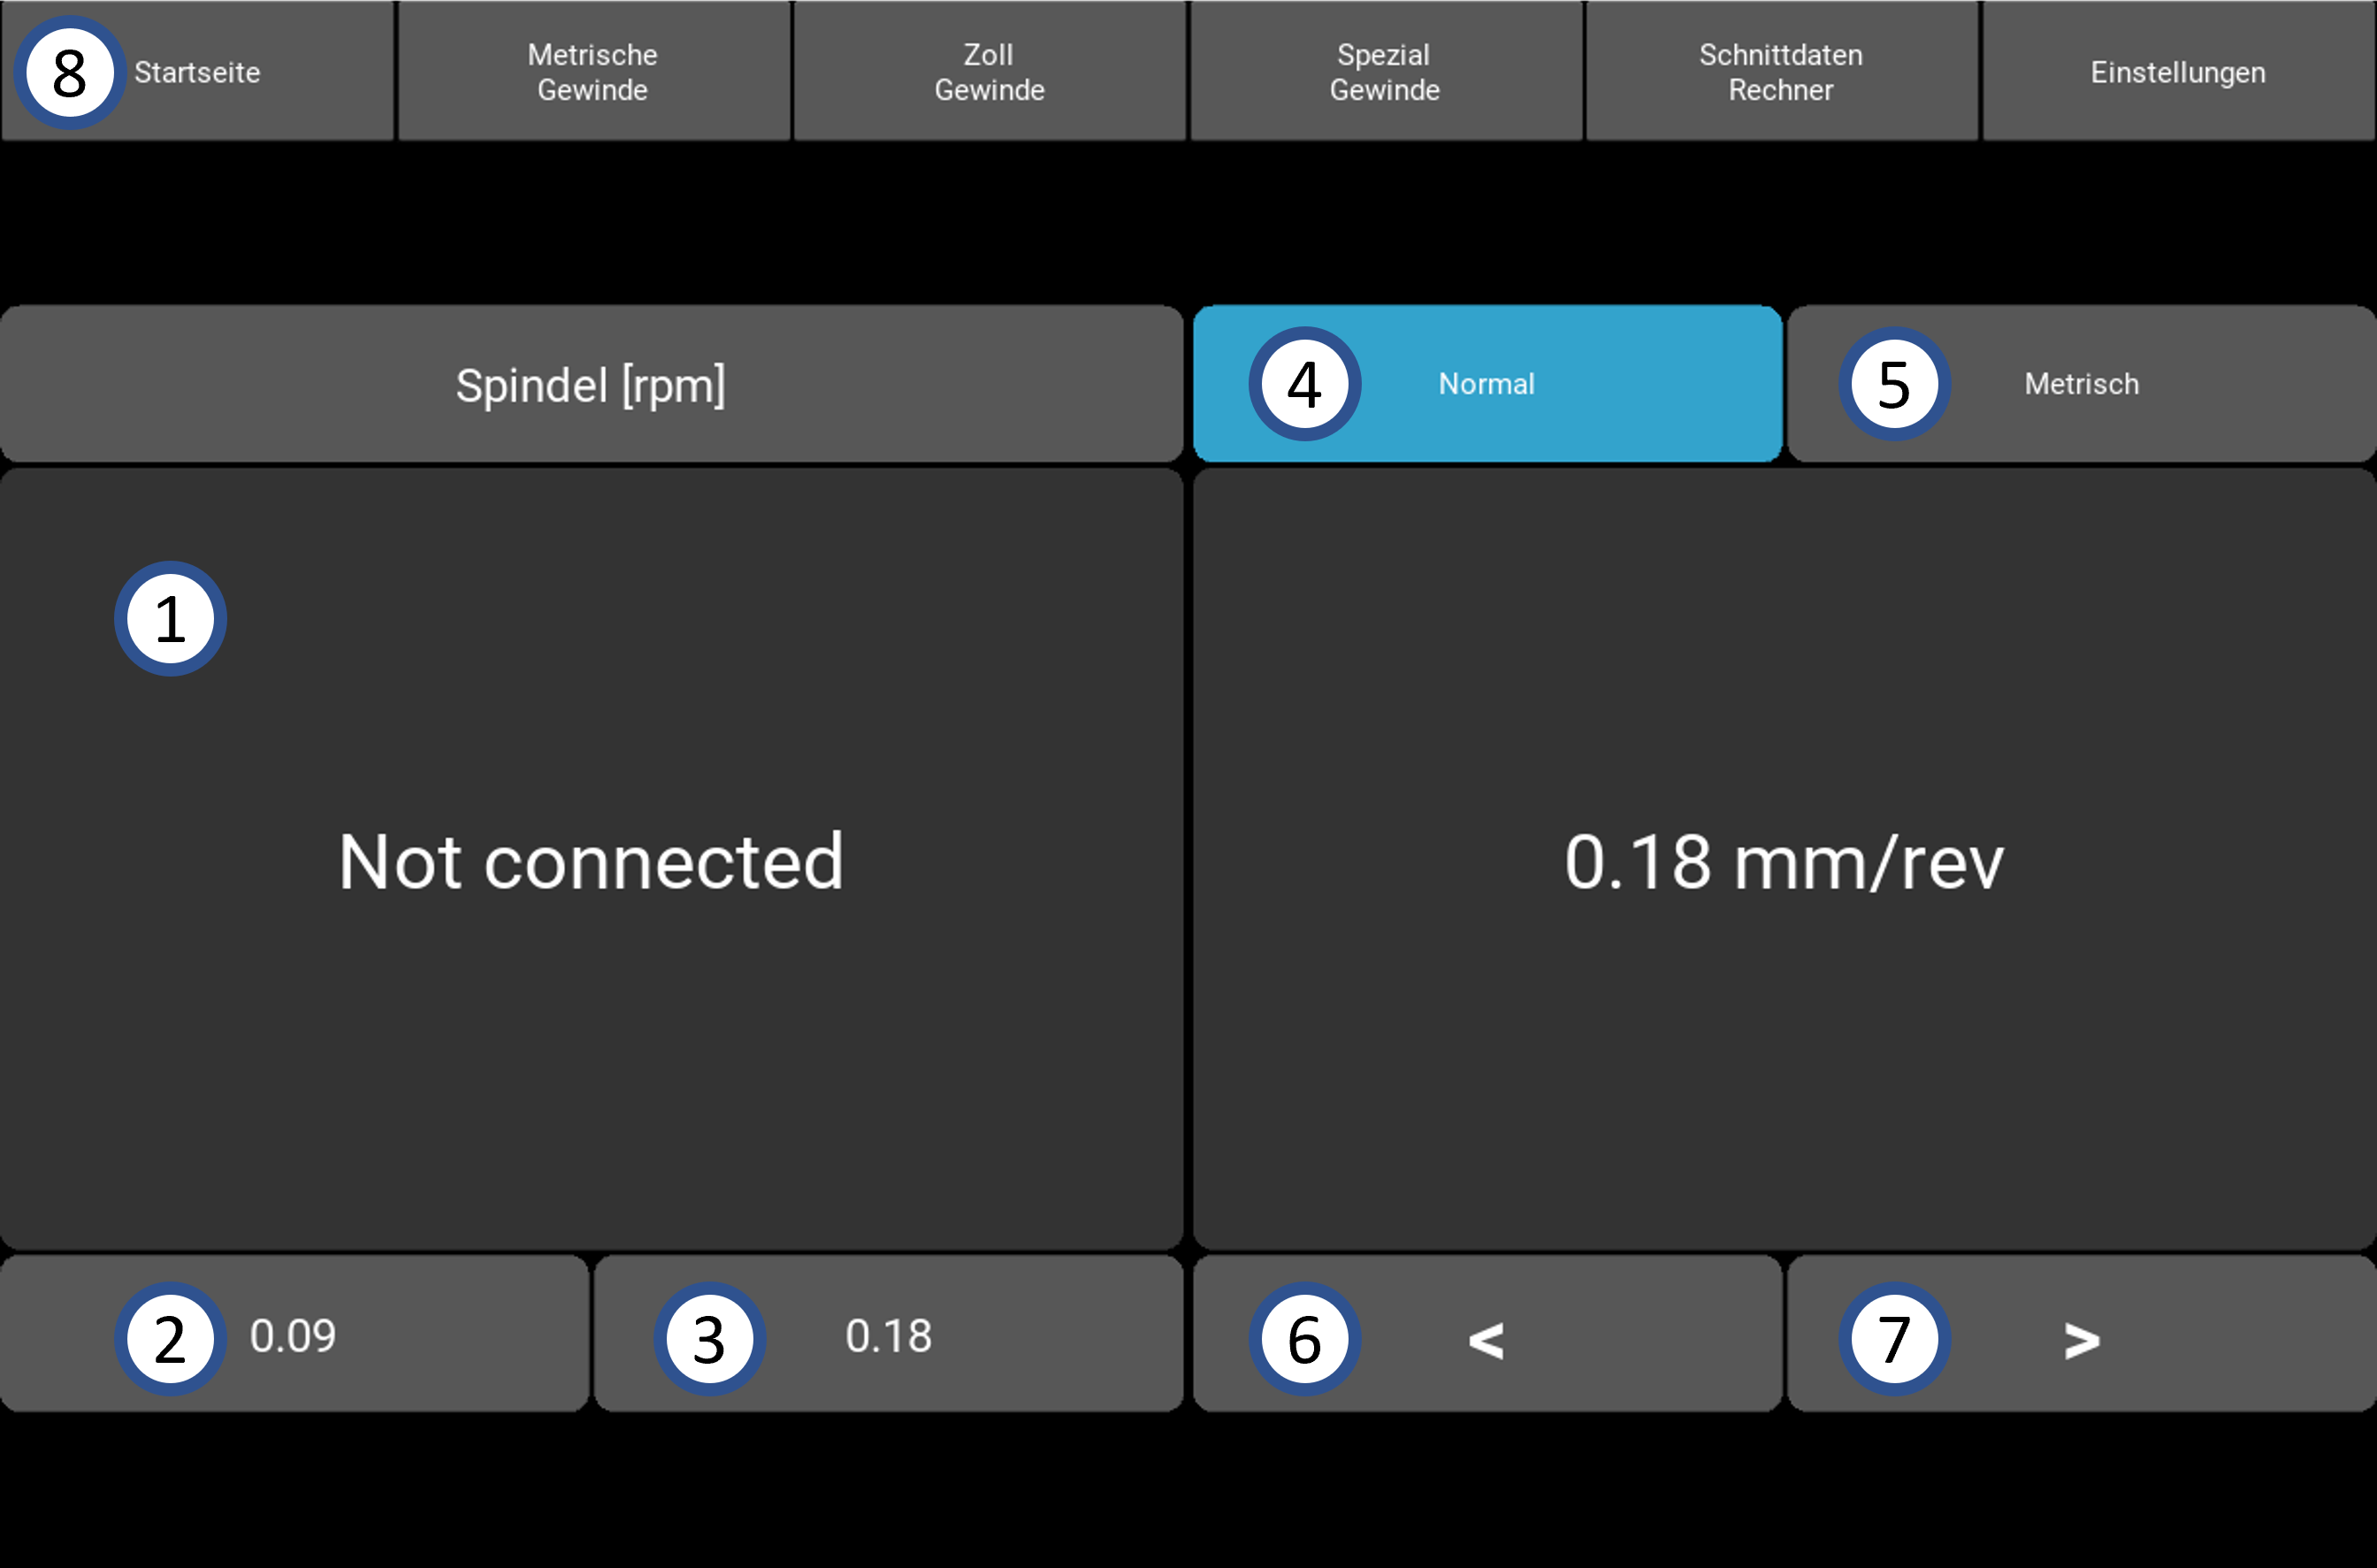
\includegraphics[width=12cm]{Pictures/HMI.png}
    \caption[Picture of the main HMI screen]{Picture of the main HMI screen; 1 - Main spindle rpm display, 2+3 - Shortcuts to most common feed rates, 4+5 - Mode selection, 6 - Step back, 7 - Step forward, 8 - Submenus}
    \label{HMI main Screen}
    \end{center}
\end{figure}

\subsubsection{Micro Controller}
The first step of the design of the micro controller was its selection. This was done based on the requirements and the work of James Clough. As a result, the micro controller platform TI LaunchXL F280049C was selected. Because of the Matlab support and the hardware ports for encoder, this was a perfect match for this project.\\
The software for the Texas Instruments micro controller was developed in two parts. First, detailed block diagram of the intended function of the software was created. This was done to keep the structure of the software as simple as possible. As shown in Figure \ref{MicroContBlockDia}, the functional software, running on the micro controller is build around two main functions. The first function calculates the number of desired steps based on the steps generated by the encoder on the main spindle. The second function generates the motor control signals. These are represented by a logical signal for the intended motor direction and a logical puls with a width of 1$\mu$s and a duty cycle of 50\%. These actions need to be performed in realtime. This means that those functions need to be executed cyclic within a certain time limit, the so called "real time requirement". In the case of the ELS, the real time requirement is the 1$\mu$s pulse length that is needed for the motor signal. However, this time frame is so short that the micro controller could not execute both functions within the given realtime requirement. For this reason two real time loops were created, one with a 100ms cycle time to calculate the Desired Steps, the other with a 1$\mu$s cycle time to generate the motor pulses. These functions work with a shared memory the "step backlog". Everytime the calculation of the desired steps is done, the steps in the backlog are incremented. Whenever the pulse function is finished with one pulse the step backlog is decremented.\\ 


\begin{figure}
    \begin{center}
    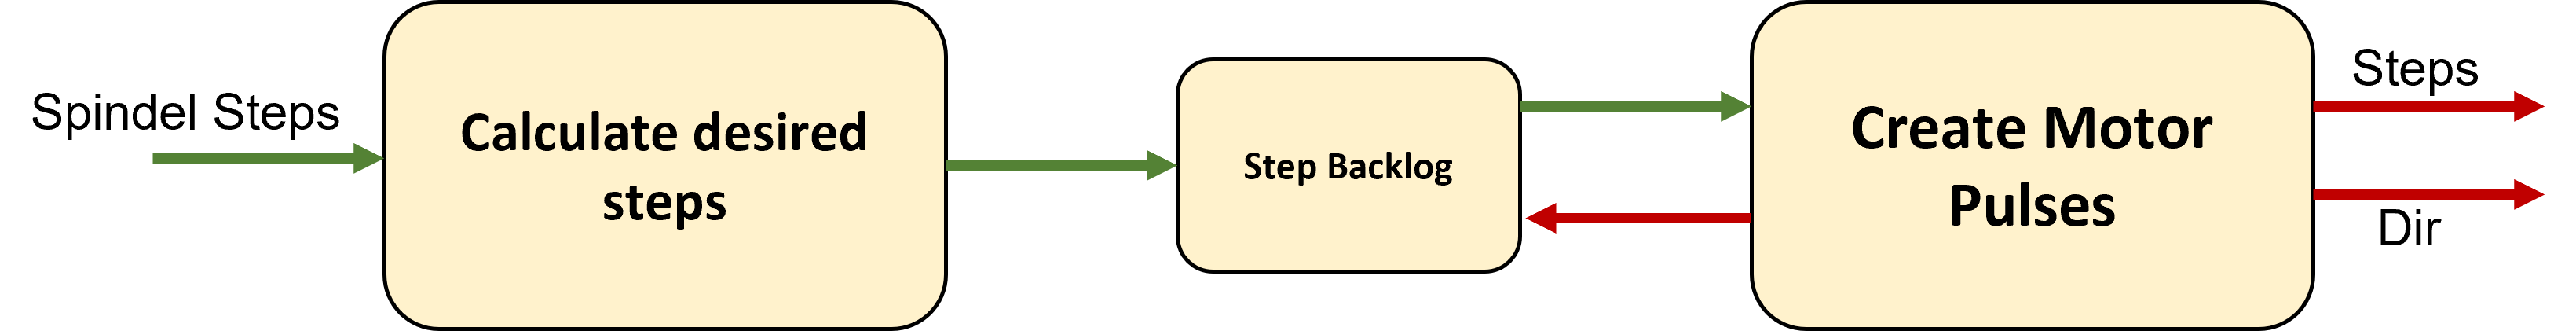
\includegraphics[width=12cm]{Pictures/MicroContBlockDia.png}
    \caption[Block diagram of the functional software on the TI Launchpad]{Block diagram of the functional software on the TI Launchpad}
    \label{MicroContBlockDia}
    \end{center}
\end{figure}

In the second part of the software developement the previously discussed steps were translated into a Matlab-Simulink Model. This had two big advantages: First, in addition to the software model, it is possible to model the complete electromechanical system of the ELS. This is very helpful while testing and debugging the developed code. Second, it is possible to generate C code for the Texas Instruments micro controller directly from the Simulink Modell. This function code is than guaranteed to work in the exact same way it did in the model environment inside of Simulink when implemented correctly. In Figure \ref{Simulink Model} the complete Simulink Model is shown.

\begin{figure}
    \begin{center}
    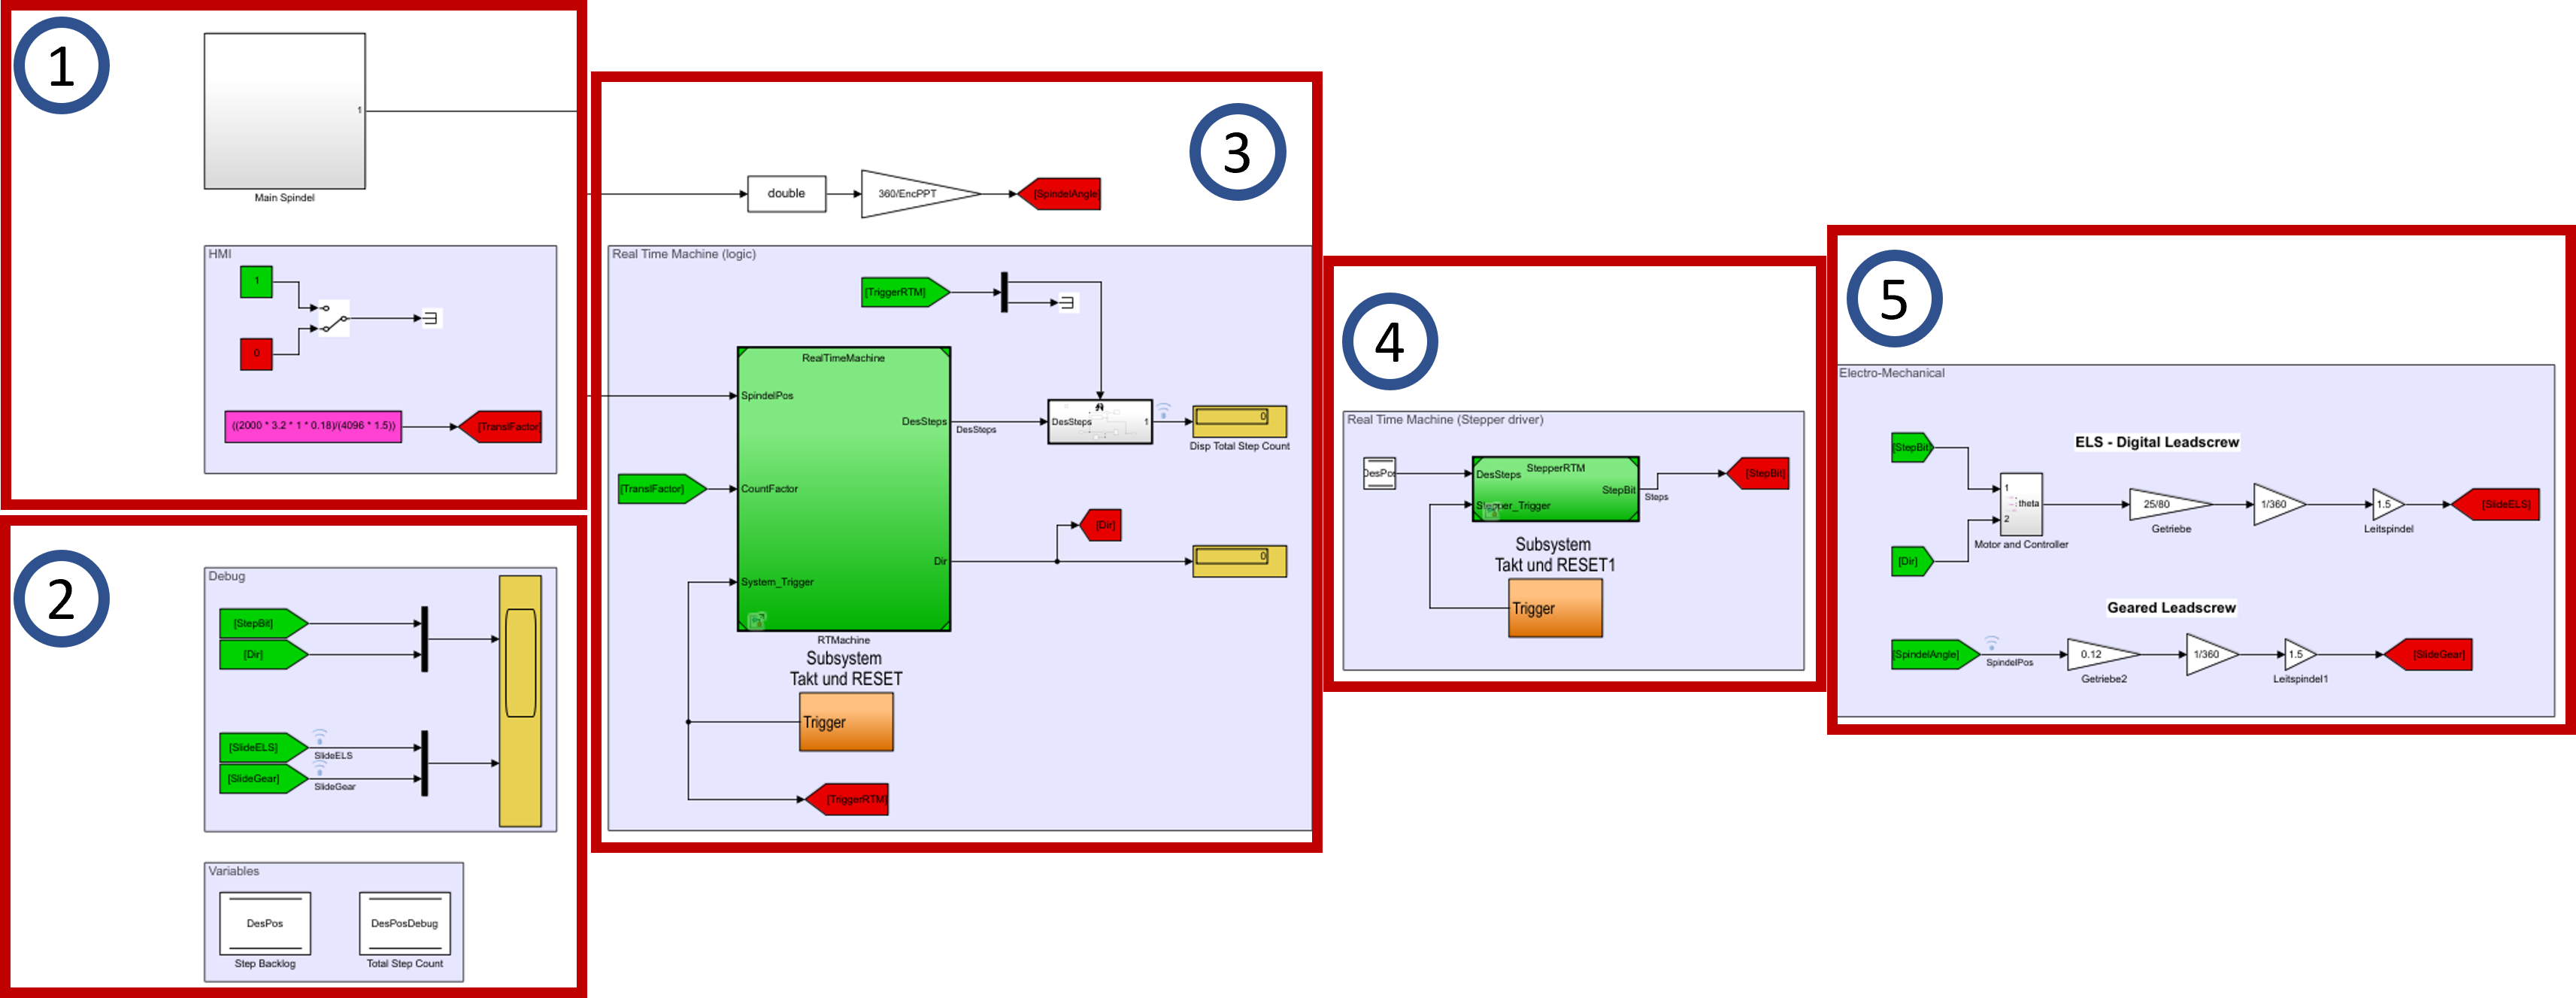
\includegraphics[width=12cm]{Pictures/SimulinkModell.png}
    \caption[Picture of the created Simulink Model]{Picture of the created Simulink Model; 1 - Model of the Spindel and the Encoder, 2 - Outputs of the Model, 3 - Model of the function calculating the desired Steps, 4 - Model of the function generating the motor pulses, 5 - Model of the Leadscrew with ELS and with the original drive train}
    \label{Simulink Model}
    \end{center}
\end{figure}


\subsubsection{Encoder}
%%TODO Put Opkon in Appendix List of Companies
The design or in this case selection of the encoder was purely based on the previously defined requirements. The most significant requirements are shown in Table \ref{Tab Encoder Key Requirements}.

\begin{table}
    \centering
     \begin{tabular}{||c|c|c||} 
        \hline
        Req. Nr. & Requirement & Value\\ [0.5ex] 
        \hline\hline
        1 & Physical Size       & 60mm		\\ 
        2 & Supply Voltage      & 5V        \\
        3 & Resolution          & 4096 ppt  \\
        4 & Directional         & Yes       \\[1ex] 
        \hline
     \end{tabular}
     \caption{Selection of Key Requirements for the ELS}
     \label{Tab Encoder Key Requirements}
\end{table}

This lead to the selection of a Encoder from the manufacturer Opkon (see Appendix \ref{AppendixListOfCompanies}). The Encoder creates 4096 pulses/revolution, with half of them phase shifted by 90\degree in order to determine the turning direction. Further, the encoder covers an input voltage range from 5V - 30V, which is compatible with the Encoder Pins on the Launchpad XL. With a hight of 57mm, the Encoder just fits into the previously determined specifications.

\subsubsection{Motor and Motor Controller}
%%TODO Put Steppers Online in Appendix List of Companies
The motor was selected based the requirements list as well as recommendations from James Clough \cite{CloughELS}. The selected motor is from the company Steppers Online (see Appendix \ref{AppendixListOfCompanies}). It is a so called "integrated servo moter". This means, the motor consist of a brushless DC-motor, an encoder as well as the corresponding motor controller. All three of these parts are packaged into one unit as shown in Figure \ref{Integrated Servo Motor}.\\

\begin{figure}
    \begin{center}
    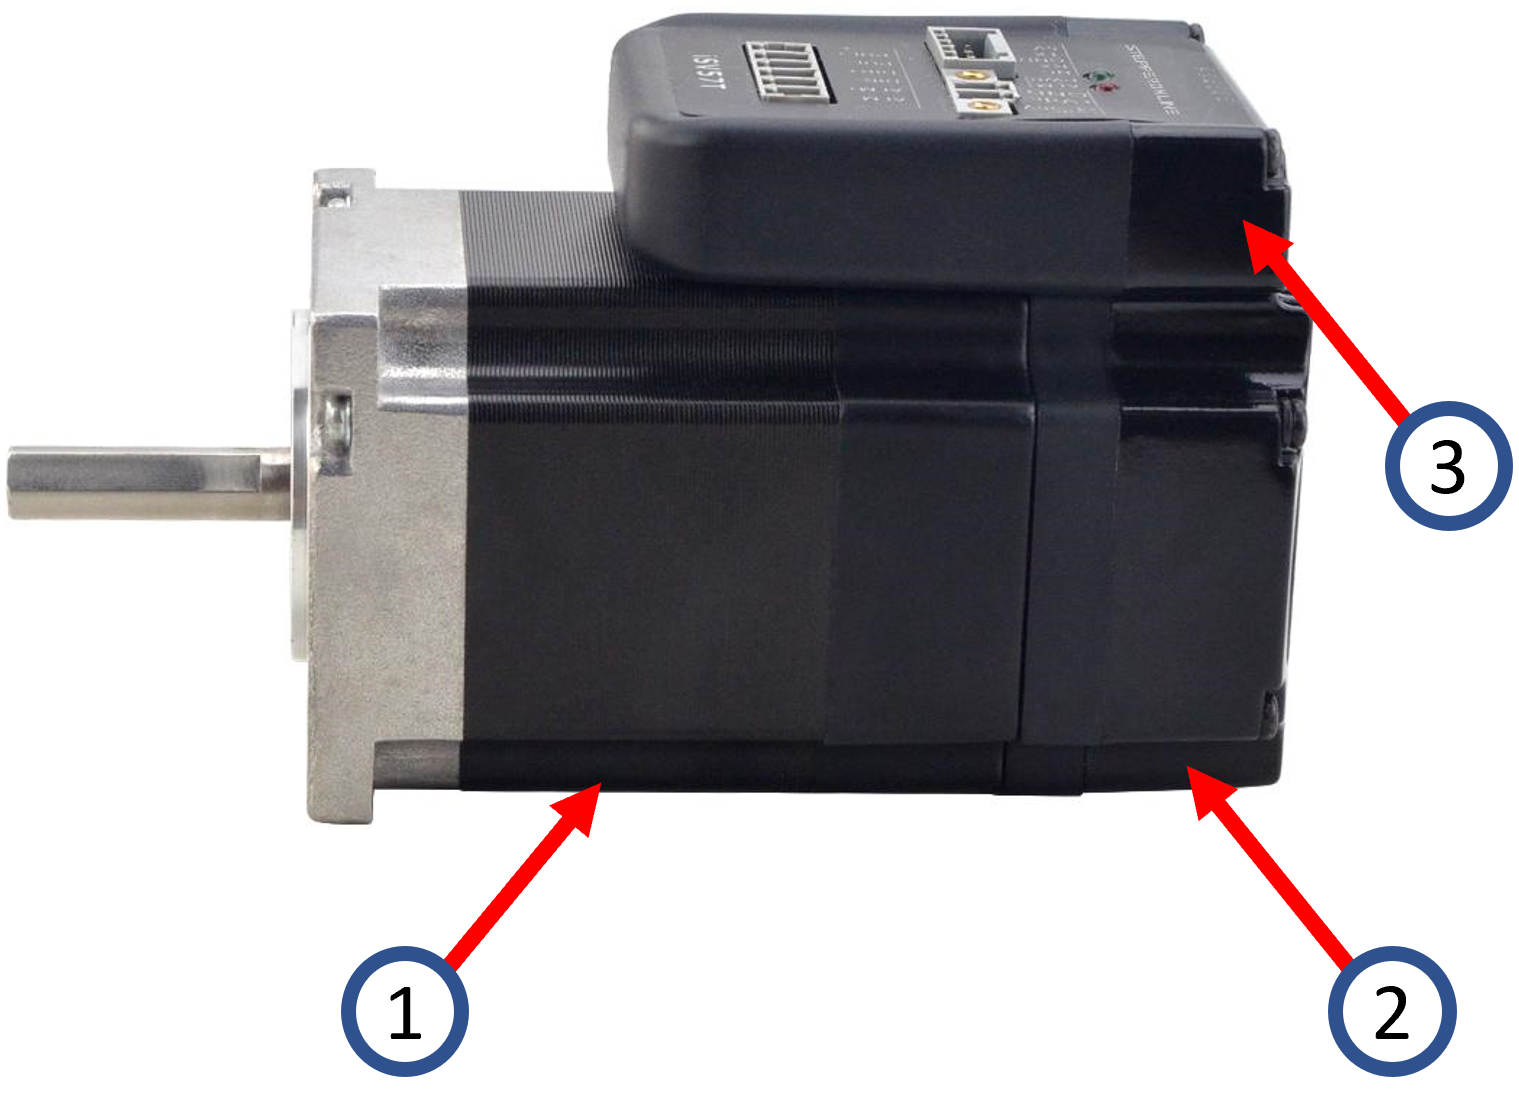
\includegraphics[width=12cm]{Pictures/IntegratedServo.png}
    \caption[Integrated Servo Motor]{Integrated Servo Motor; 1 - BLDC Motor, 2 - Encoder Unit, 3 - Control Unit}
    \label{Integrated Servo Motor}
    \end{center}
\end{figure}

The motor features an RPM range from 0 to 4000 rpm and a very constant maximum torque of 0.4 nm. Further, it has the right dimensions in order to fit the space claim requirements.\\
The motor controller in combination with the required software represent an easy programming interface. Via this interface, control parameters as well as parameter for the dynamics and precision of the motor can be set. As a starting value, the motor stiffness (responsiveness) gain was set to its maximum. Based on the software design of the micro controller, the precision of the motor was set to 2000 steps/revolution.\\
The interface to the motor is provided by a simple digital protocol. It consists of a direction and a step pin. The direction reacts to a logical 5V signal, where a logical 1 (5V) corresponds to clockwise rotation and a logical 0 (0V) corresponds to counterclockwise rotation. The step input reacts to logical pulses with a minimum pulse width of 1$\mu$s. Each puls will than move the motor by $\frac{1}{motor-resulution}$.

\subsubsection{Gearbox}
Because the motor is mounted underneath the Leadscrew, a a coupling between both elements was needed. This was done with the already existing gears from the old gearbox of the lathe. This decision was made because it needed the least modification (only a coupler from the motor to the gear had to be manufactured) and was the cheapest option. The gear ratio of 25/80 was selected to optimize the feed range of the lathe with the available RPM of the motor. This is shown in Figure \ref{Chart Leadscrew Dynamics}.

\begin{figure}
    \begin{center}
    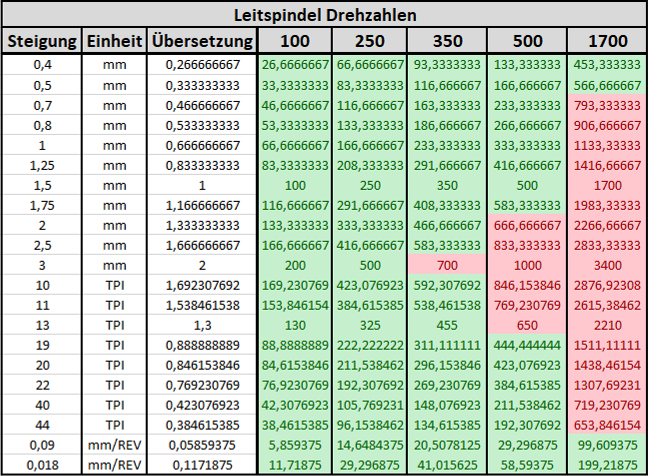
\includegraphics[width=12cm]{Pictures/TransmissionDynamics.png}
    \caption[Chart of the Leadscrew dynamics]{Chart of the Leadscrew dynamics; green - reachable Leadscrew RPM with a 25/80 transmission, red - not reachable Leadscrew RPM with a 25/80 transmission}
    \label{Chart Leadscrew Dynamics}
    \end{center}
\end{figure}

The transmission of the gearbox also increases the torque of the motor by a factor of 3.2. This way, the motor meets the specified torque of 1.2 Nm.

\subsection{Software Implementation}
The task during the implementation of the software was to deploy the developed code the the according hardware. Further, the communication between the HMI and the real time controller needed to be established.
\subsubsection{Micro Controller}
The implementation of the software design for the micro controller was one of the biggest tasks during the developement of the Electronic Leadscrew System. It was done in multiple steps.\\
First the functional part of the software was created using Matlab and Matlab Simulink. In the functional software, a series of logical actions were needed in order to compute the required motor signal based on the the encoder position.
The task of the first software part was it to process the position data coming from the encoder and calculate the desired motor position. This process is shown in form of a block diagram in figure \ref{Blockdia funcSoft 1}.\\

\begin{figure}
    \begin{center}
    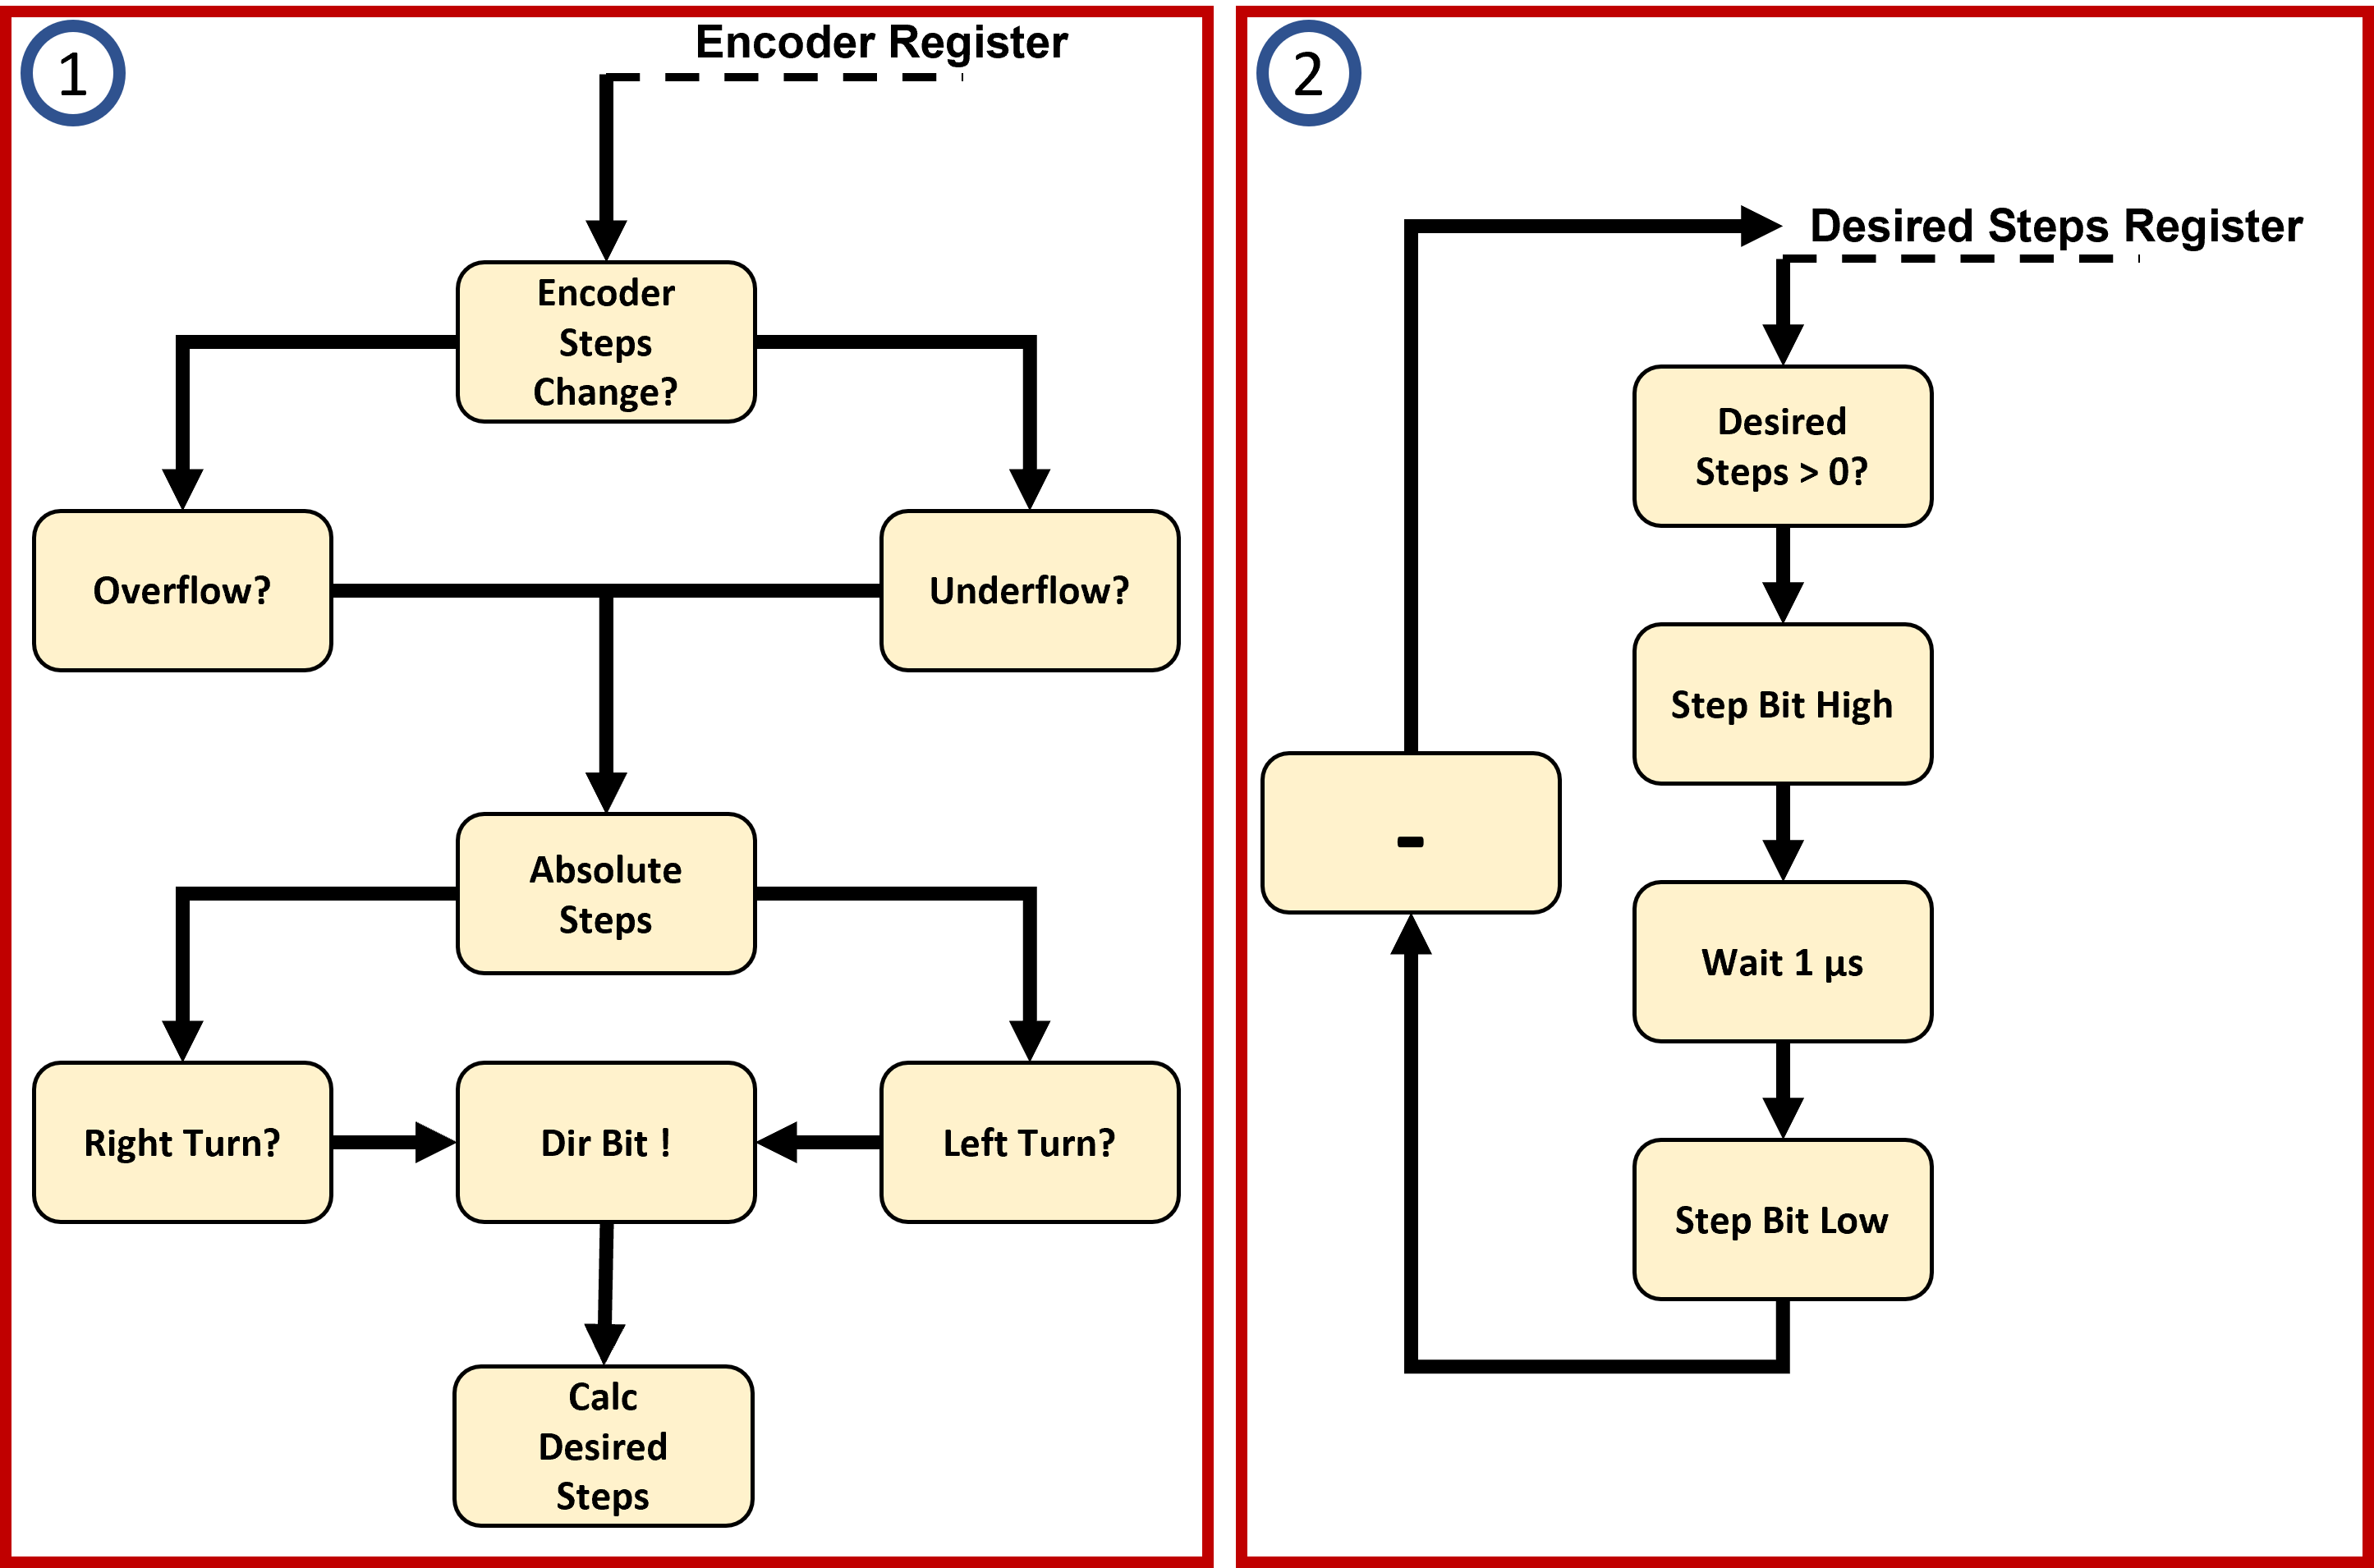
\includegraphics[width=12cm]{Pictures/funcSoft_1.png}
    \caption[Block diagram of the first part of the functional software]{Block diagram of the first part of the functional software; 1 - Functional Software first part, 2 - Functional Software second part}
    \label{Blockdia funcSoft 1}
    \end{center}
\end{figure}

Because the encoder is constantly incrementing the value of a 16bit register, it is possible that the value reaches the maximum or minimum possible value. In this case, the register value will "overflow" and jump from its maximum to its minimum or from its minimum to its maximum value. This would result in a very big but wrong movement of the motor. The first step of the functional software is to detect such an overflow and correct for it. This way the calculation of the desired steps is always performed with the absolute movement of the encoder. Next, the direction of rotation of the spindle needs to be detected and the direction output to the motor need to be set accordingly. In the last step of the functional software the desired steps are calculated. This is done by multiplying the steps of the encoder by a previously determined translation factor.\\

The second part of the functional software generates the logical pulses in order to move the motor. Therefore it checks the register value of the desired steps on a cyclic basis. If this value is not zero, the software will create a one micro second logical pulse and decrement the register value afterwards by one. These steps are also shown in figure \ref{Blockdia funcSoft 1}.\\
During the second part of the software implementation, the functional code was translated to C Code using Matlabs Code generation toolbox and deployed to the hardware. To be able to use the functional code on the micro controller an implementation routine needed to be created. This routine was used in order read all inputs, such as the encoder position and th communication interface relay this information to the functional code. Further the implementation routine enabled the functional code to use the GPIO module of the micro controller and send out the current RPM of the spindle via the communication interface.

\subsubsection{HMI}
After the creation of the graphical interface during the design phase, the HMI needed to be connected to the micro controller. For this purpose a UART communication interface was used. To transmit Mode and translation factor and receive the spindle RPM simultaneously, a custom communication protocol was created. This protocol consist of 5 byte of data. The first and last byte are so called start and stop bytes, used in order to determine between different data packages. They have the value 0xFF. The second byte is an integer with a value between 0 and 2 in order to communicate normal, metric or imperical mode to the micro controller. The third and fourth bytes represent the determined translation factor. Because it is not possible to transmit fractional numbers via a UART communication interface, the integer part of the translation factor is transmitted in the third byte. The fractional value of the translation factor is then converted to an integer and transmitted in the fourth byte. This process has than to be reversed on the micro controller.

\subsection{Hardware Implementation}
For the implementation of the Hardware, the main task was to solve mechanical problems. This was done with the extensive use of a CAD Software, a 3-D Printer as well as the Lathe.

\subsubsection{Touchscreen}
In order to mount the touchscreen as well as the Raspberry Pi to the lathe, a housing needed to be created. This was done by first modeling each of the components as well as a section of the lathe in the CAD Software Autodesk Fusion 360. After this, a house was created the positioned the touchscreen in a way that made it convenient to read and operate while working on the lathe. Further, the housing featured an enclosure for the Raspberry Pi that was mounted to the back of the touchscreen.

\begin{figure}
    \begin{center}
    \includegraphics[width=12cm]{Pictures/touchscreenImp.png}
    \caption[Cross section of the Touchscreen mount]{Cross section of the Touchscreen mount; 1 - Touchscreen, 2 - Raspberry Pi, 3 - Enclosure and mount, 4 - Lathe model, 5 - Picture of the finished implementation}
    \label{touchscreenImp}
    \end{center}
\end{figure}

After the 3-D Model of the touchscreen mount was complete, it was 3-D printed in PETG plastic. Finally, the touchscreen could be mounted to the lathe. The 3-D model and the final result are shown in figure \ref{touchscreenImp}.

\subsubsection{Encoder}
For the implementation of the encoder to problems needed to be solved. First, a method needed to be developed in order to mount the encoder to the lathe. Second, the RPM of the main Spindle needed to be transferred to the shaft of the rotary encoder.
In order to mount the encoder to the lathe all components were modeled in Fusion 360. As a good mounting point on the lathe, the old gear holder stood out. This way the encoder position could be changed easily. In the second step the mount for the encoder was modeled as well as a gear in order to transfer the spindle RPM to the encoder with a 1:1 transmission factor. Both the holder and the gear were 3-D printed. Only the standoffs for the mount were manufactured from Aluminium on the lathe. This was done in order to insure a rigid mounting of the encoder. Figure \ref{EncoderImp} shows the complete mounting of the encoder.

\begin{figure}
    \begin{center}
    \includegraphics[width=12cm]{Pictures/EncoderImp.png}
    \caption[Image of the encoder mount]{Image of the encoder mount; 1 - Old gear holder, 2 - Machined standoffs, 3 - 3-D printed Encoder mount, 4 - Encoder model, 5 - 3-D printed gear, 6 - Picture of the finished implementation}
    \label{EncoderImp}
    \end{center}
\end{figure}

\subsubsection{Motor}
Similar to the mount of the encoder and the touchscreen, the motor mount was designed with the use of Fusion 360. Because of the very limited space on the machine this was very important. First, the parts of the Lathe that could possibly interfere with the motor or its mount were modeled. Then, the motor and the motor could be designed. The motor mount was designed, such that the play of the gears can be adjusted by sliding the motor in its mount up and down. This is shown in Figure \ref{MotorImp}. After the model of the motor mount wqs finished it was 3-D printed in order to test the fit of the mount. Initially, the motor mount was supposed to be manufactured from steel afterward but during testing the 3-D printed motor mount proofed to be rigid enough.

\begin{figure}
    \begin{center}
    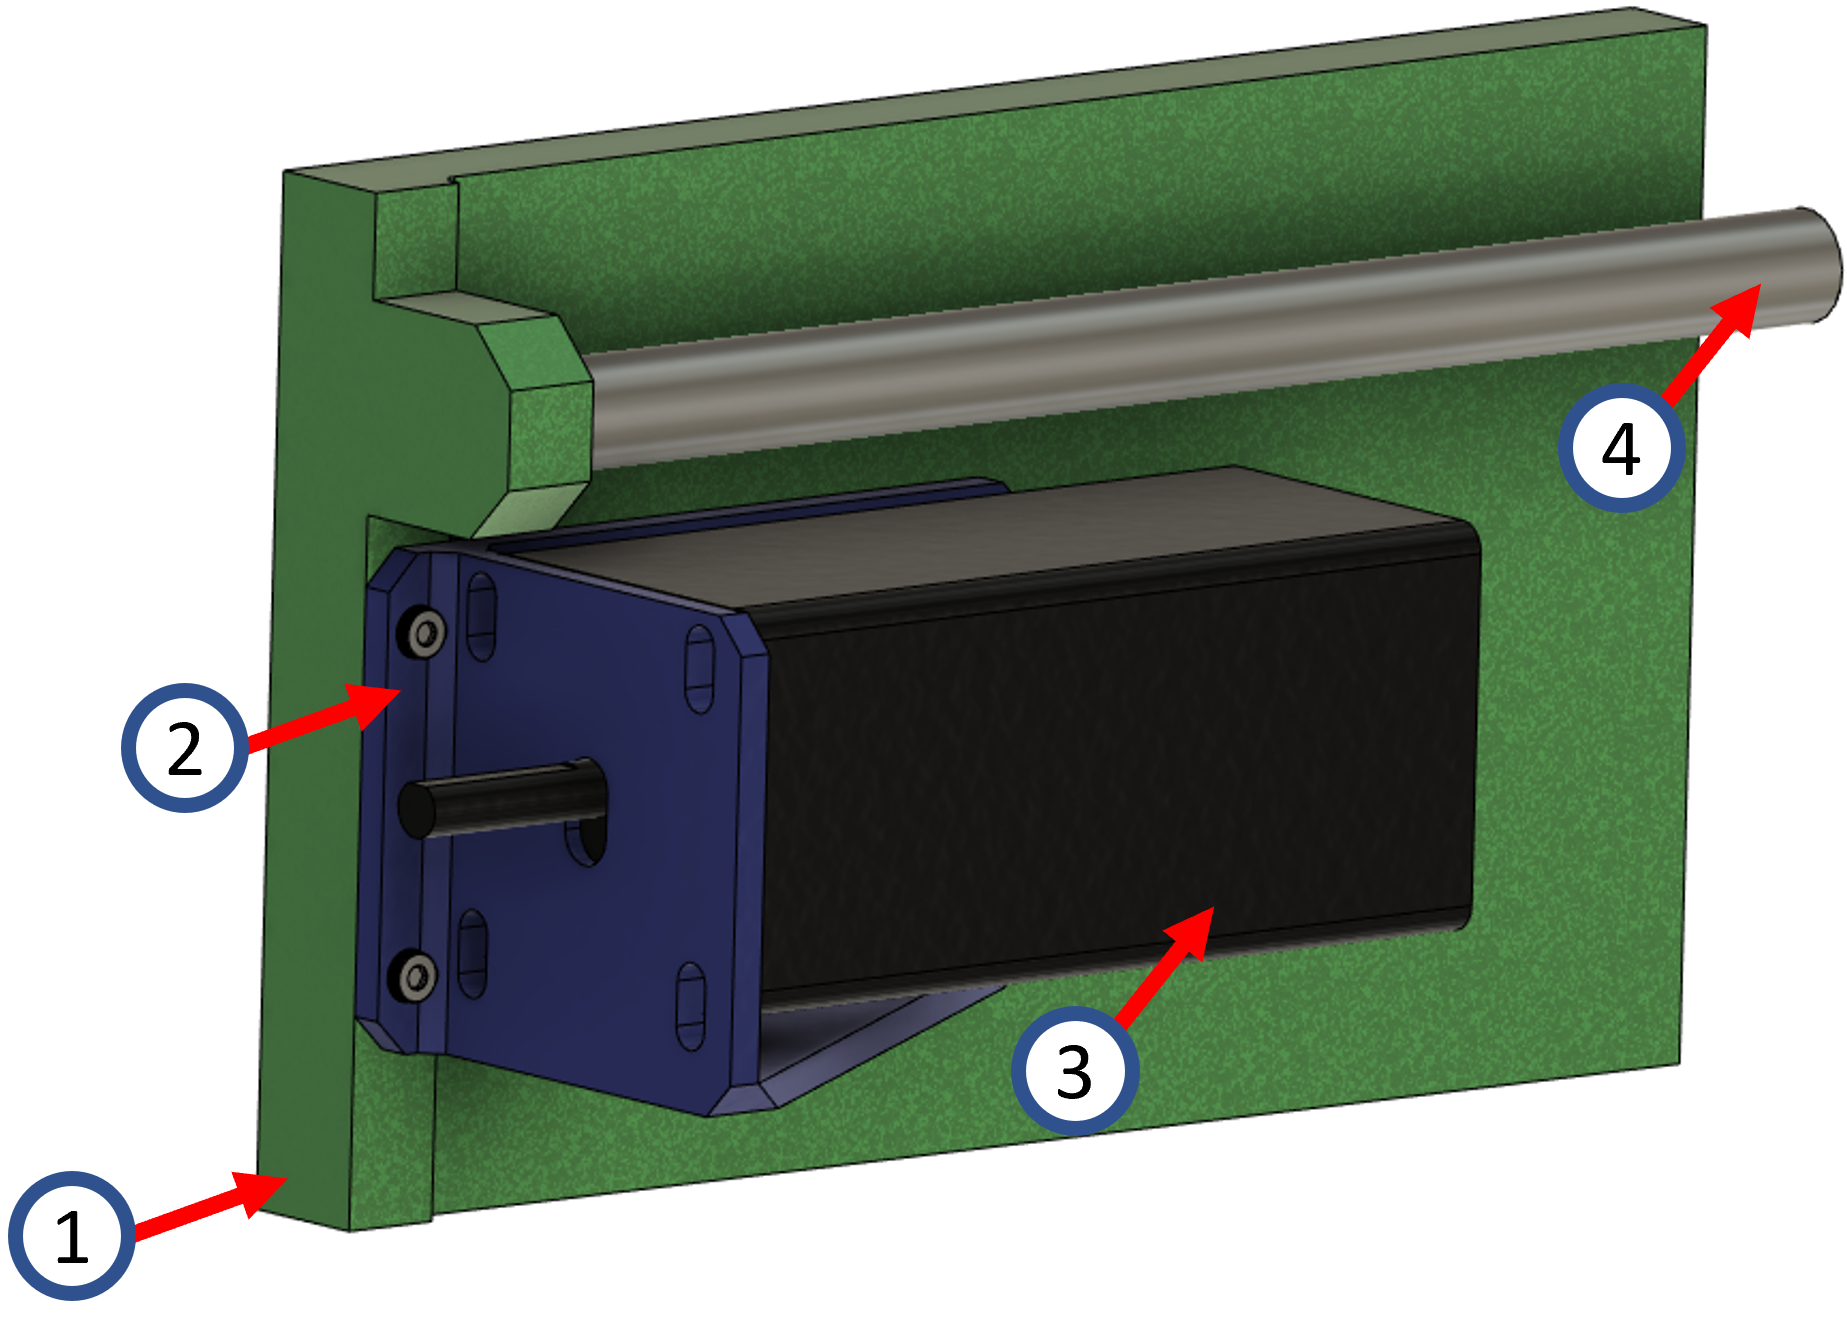
\includegraphics[width=12cm]{Pictures/MotorImp.png}
    \caption[Image of the motor mount]{Image of the motor mount; 1 - Old gear holder, 2 - Machined standoffs, 3 - 3-D printed Encoder mount, 4 - Encoder model, 5 - 3-D printed gear, 6 - Picture of the finished implementation}
    \label{MotorImp}
    \end{center}
\end{figure}

\section{Testing}
During the testing phase of the developement process, every part of the system is tested to see if it is functioning as defined in the requirements and the System design. This is done on component level, system level and finally on the Integrated system. As shown in Figure \ref{V Model Component Test}, this is the second part of the V Model developement cycle.

\begin{figure}
    \begin{center}
    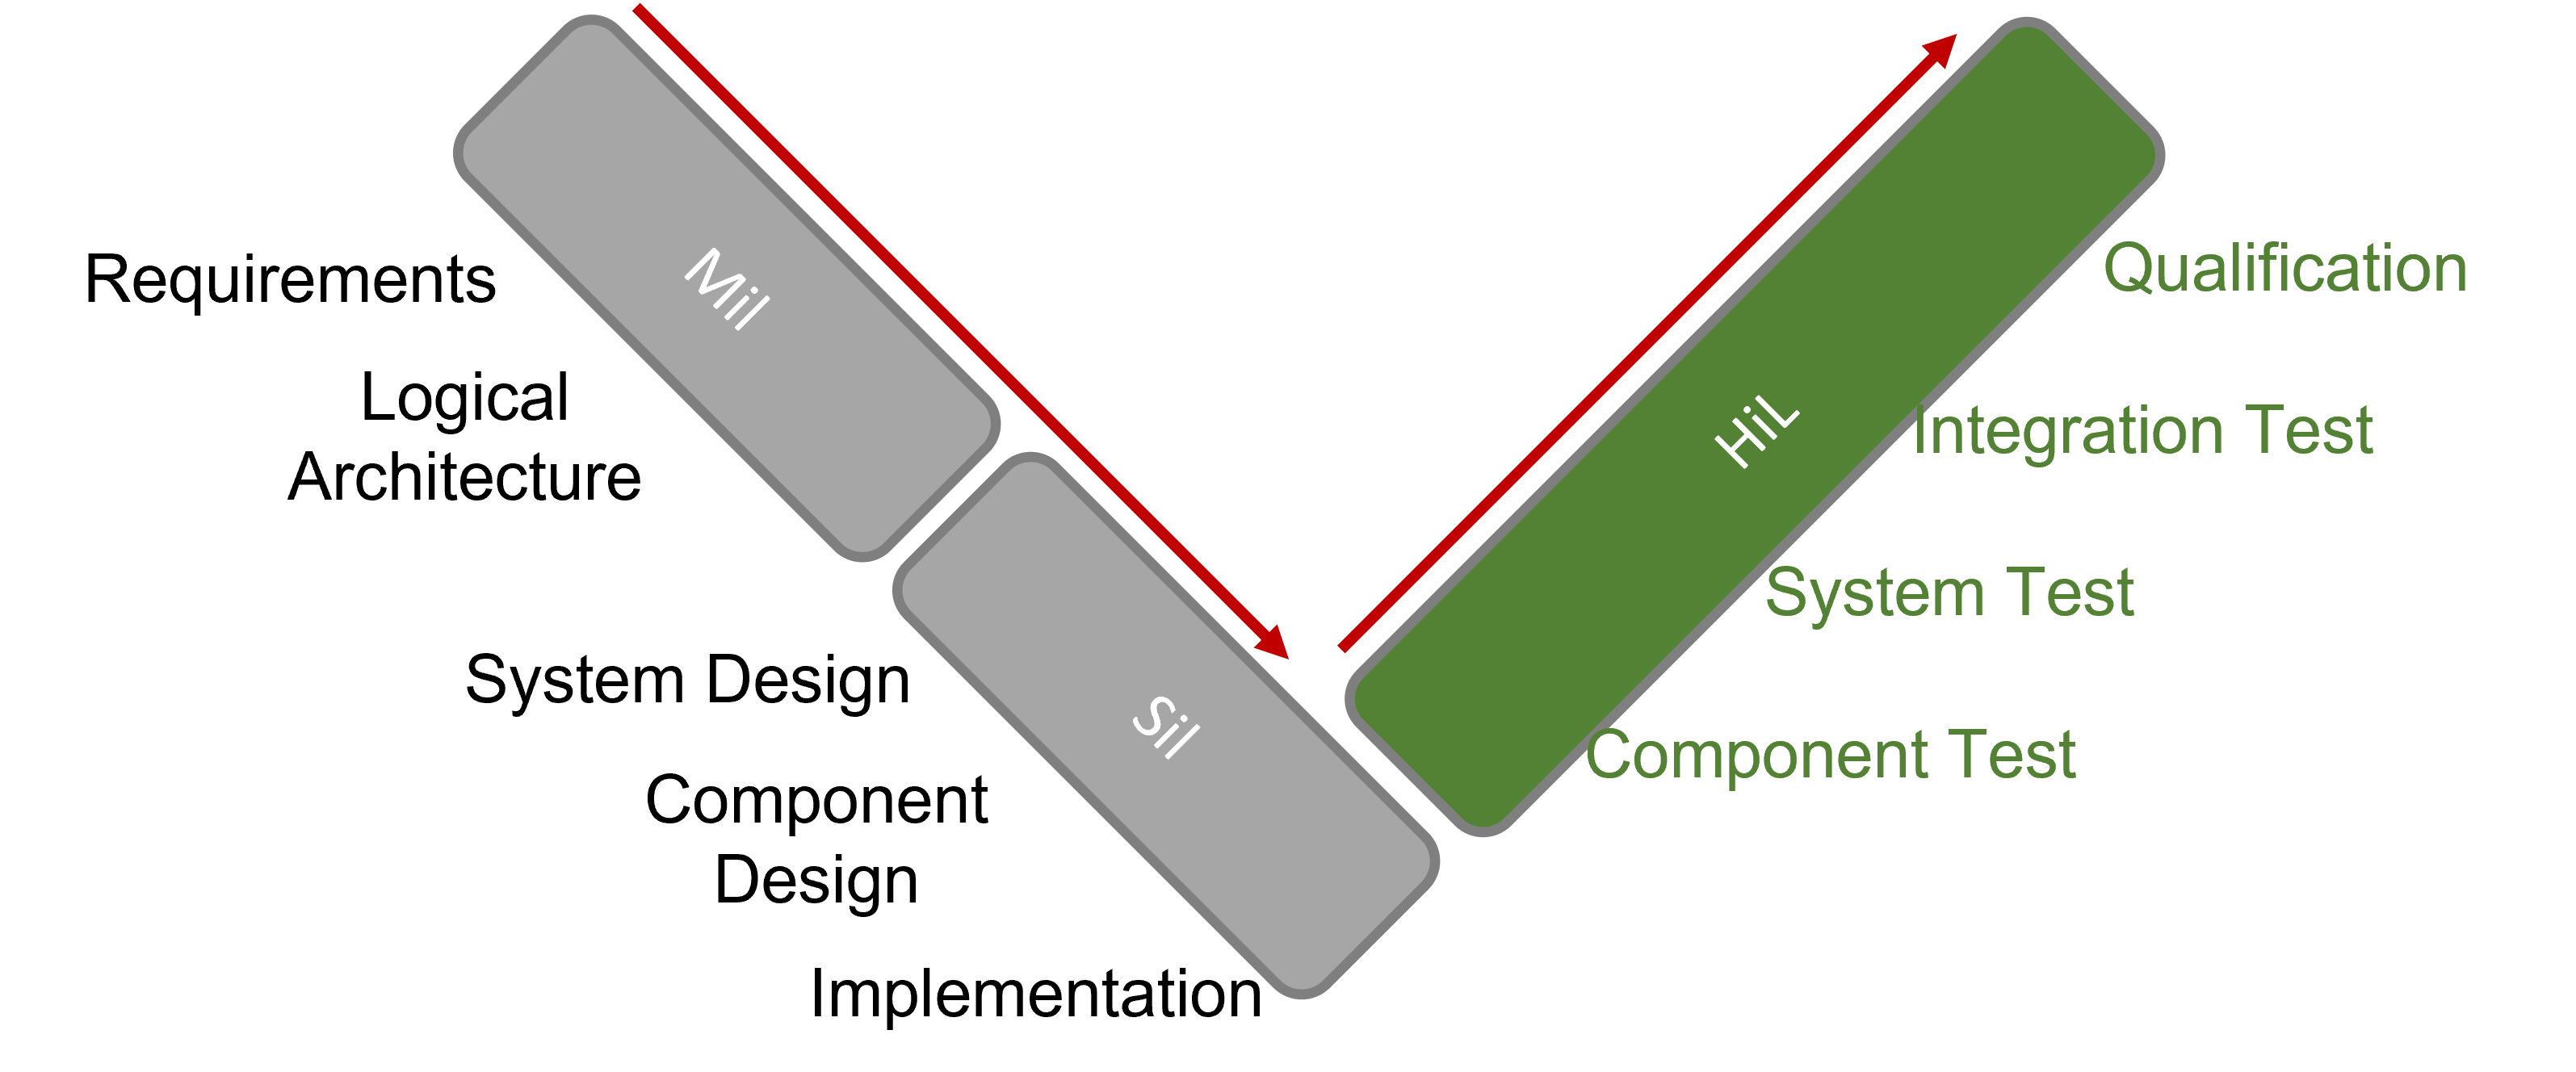
\includegraphics[width=12cm]{Pictures/V Model Component Test.png}
    \caption[V Model Component Test]{V Model Component Test Stage}
    \label{V Model Component Test}
    \end{center}
\end{figure}

\subsection{Component Test}
First the correct function of each of the components needs to be ensured. This can be done on the finished system but is often easier to do before the implementation. 
Because motor, motor controller and encoder are bought from a third party, they are not included in the component testing.

\subsubsection{HMI}
In order to test the functionality of the HMI and especially the communication a special test program was created. This program allowed to monitor the data packages send by the HMI. Further, it was possible to send RPM data to the HMI in order to test the RPM display.

\subsubsection{Micro Controller}
During the component testing phase, only the implementation softer on the micro controller was tested. This step was tremendously simplified by the onboard debugging probe of the TI LAUNCHXL developement board. This way it was able to track every register value on the micro controller to ensure a correct working behavior.
The correct timing of both real time loops were checked by toggling one of the GPIO Pins of the micro controller and reading its value with the help of an Oscilloscope.


\subsection{System Test}
The system testing was done in two stages, the first testing series was done within Matlab Simulink. Secondly the on a test bench assembled system was tested. Later the result of both test could be compared.

\subsubsection{Matlab Simulink}
In order to test the system in Matlab Simulink every component needed to be modeled. The most complex part to model in the Simulink environment was the encoder and the drive train for the Leadscrew.\\
The model of the encoder needed to be able to simulate events like an register overflow, different trajectories as well as constant speeds. The model of the encoder is shown in Figure \ref{SysEnc}.

\begin{figure}
    \begin{center}
    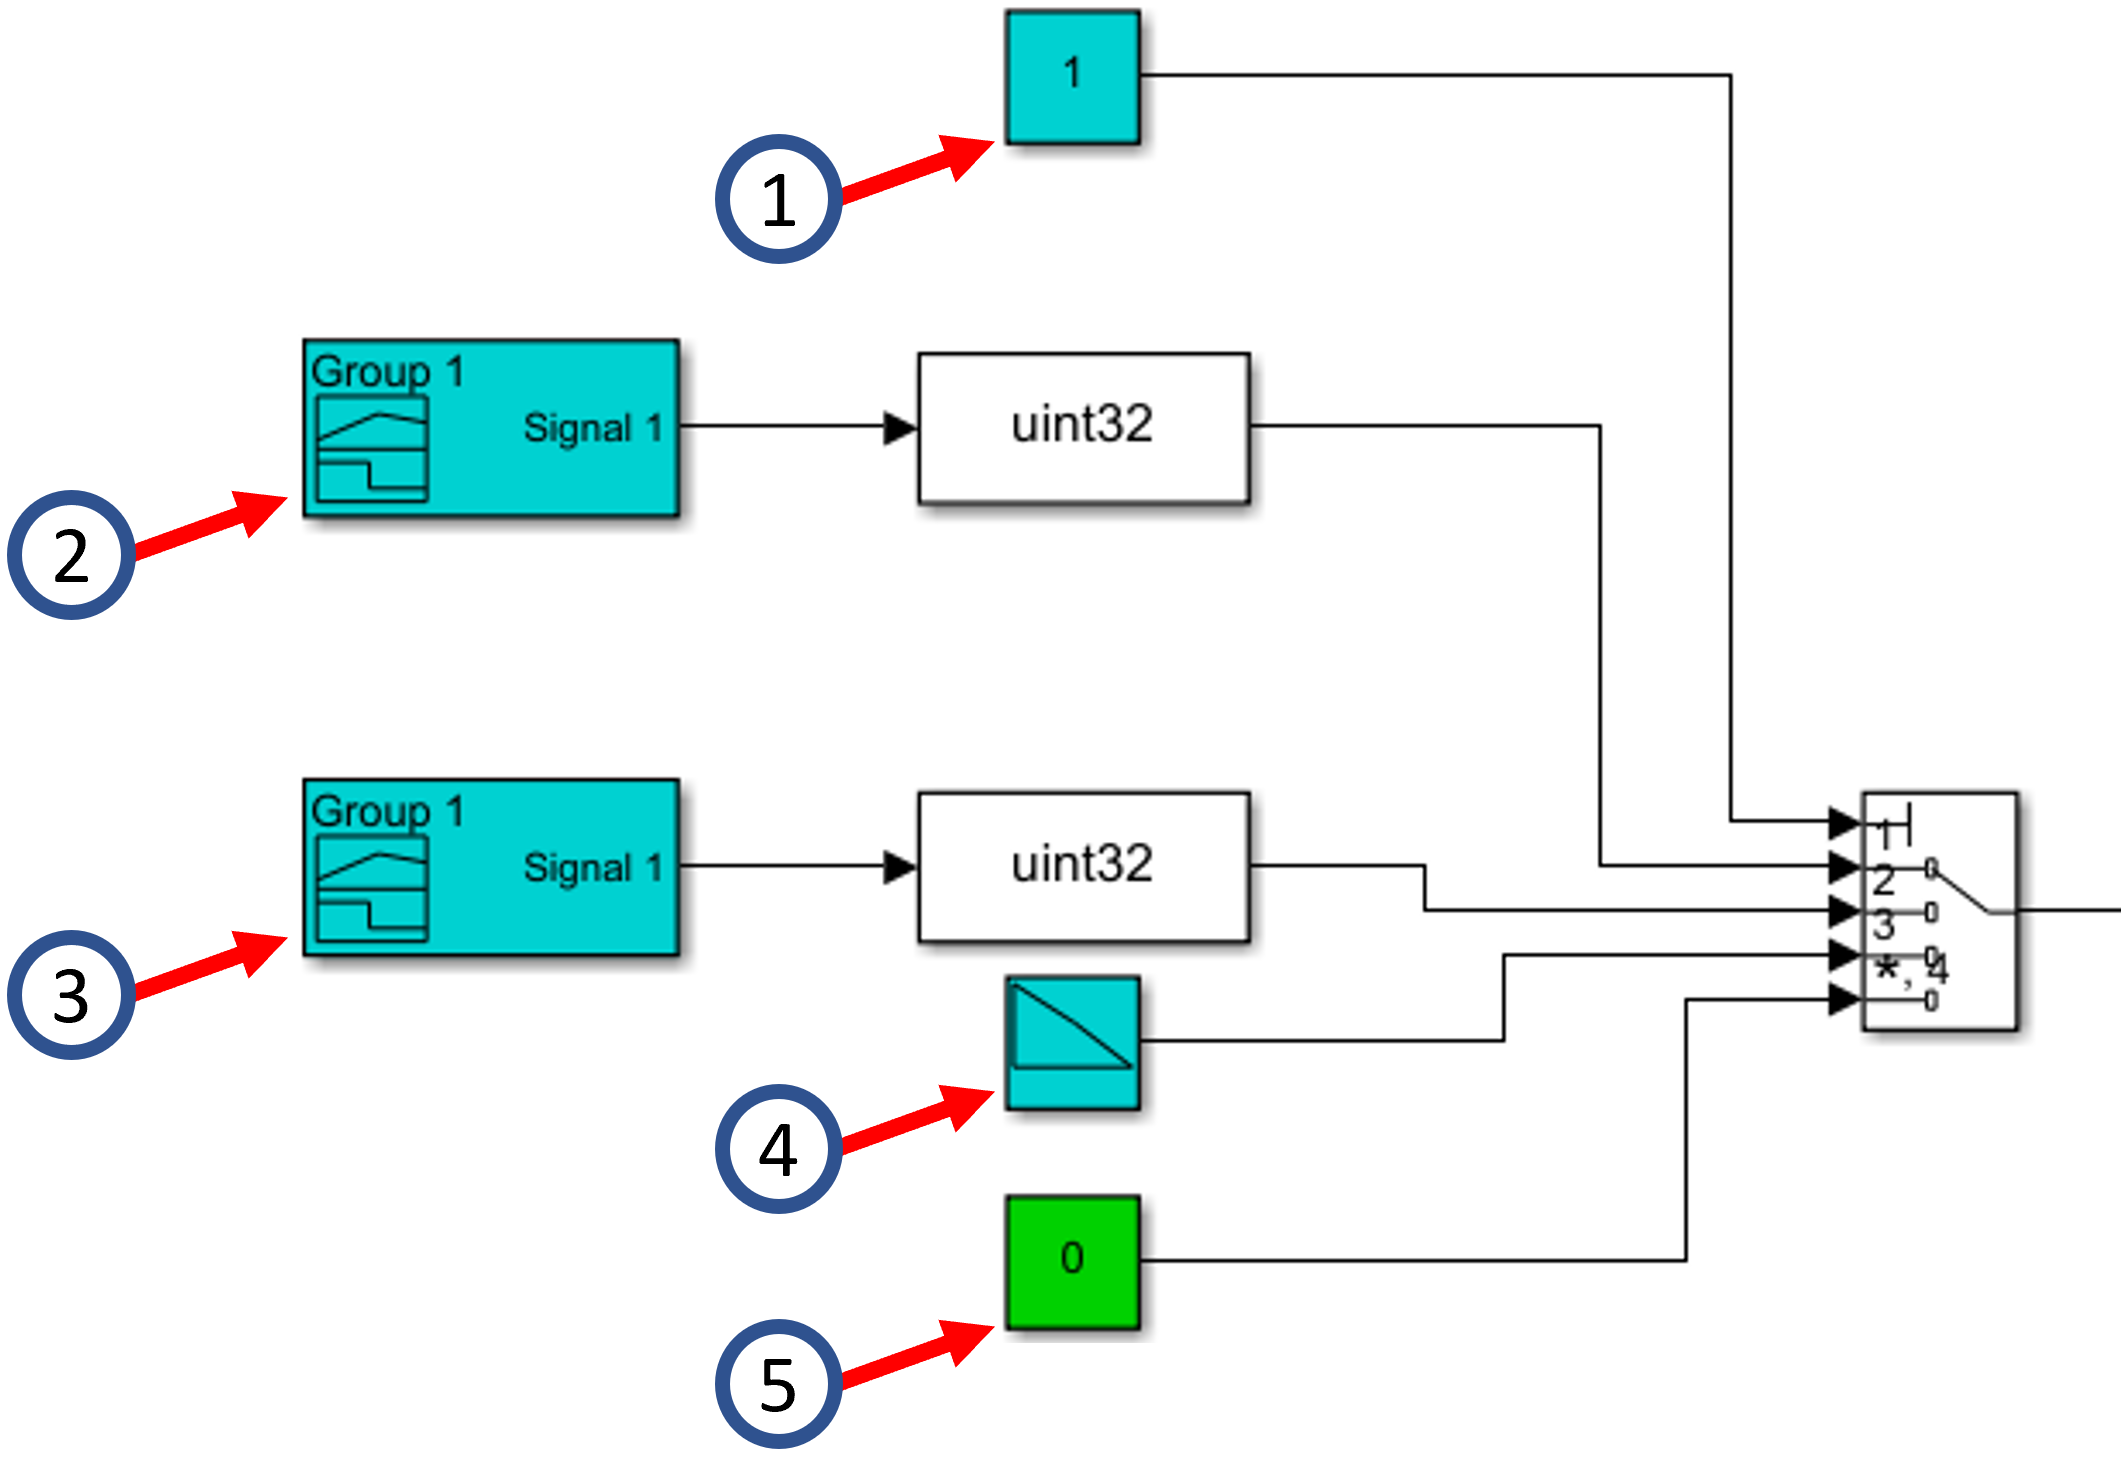
\includegraphics[width=12cm]{Pictures/SysEnc.png}
    \caption[Simulink Model of the encoder]{Simulink Model of the encoder; 1 - Constant position, 2 - Trajectory 1, 3 - Trajectory 2, 4 - Register overflow, 5 - Case selector}
    \label{SysEnc}
    \end{center}
\end{figure}

Every test function of the encoder was than routed over a case sensitive switch. This switch can be controlled by a variable and connects based on this on input to the output. This makes switching the test scenario easy and fast.\\

For the simulation of the drive train both the electronic and the original gear drive train were modeled. The motor and motor controller were modeled with a library of Simulink called "Simscape". Simscape is designed in order to model complex electromechanical with minimum effort. The model of the electronic drivetrain is shown in Figure \ref{SysEDriveT}.

\begin{figure}
    \begin{center}
    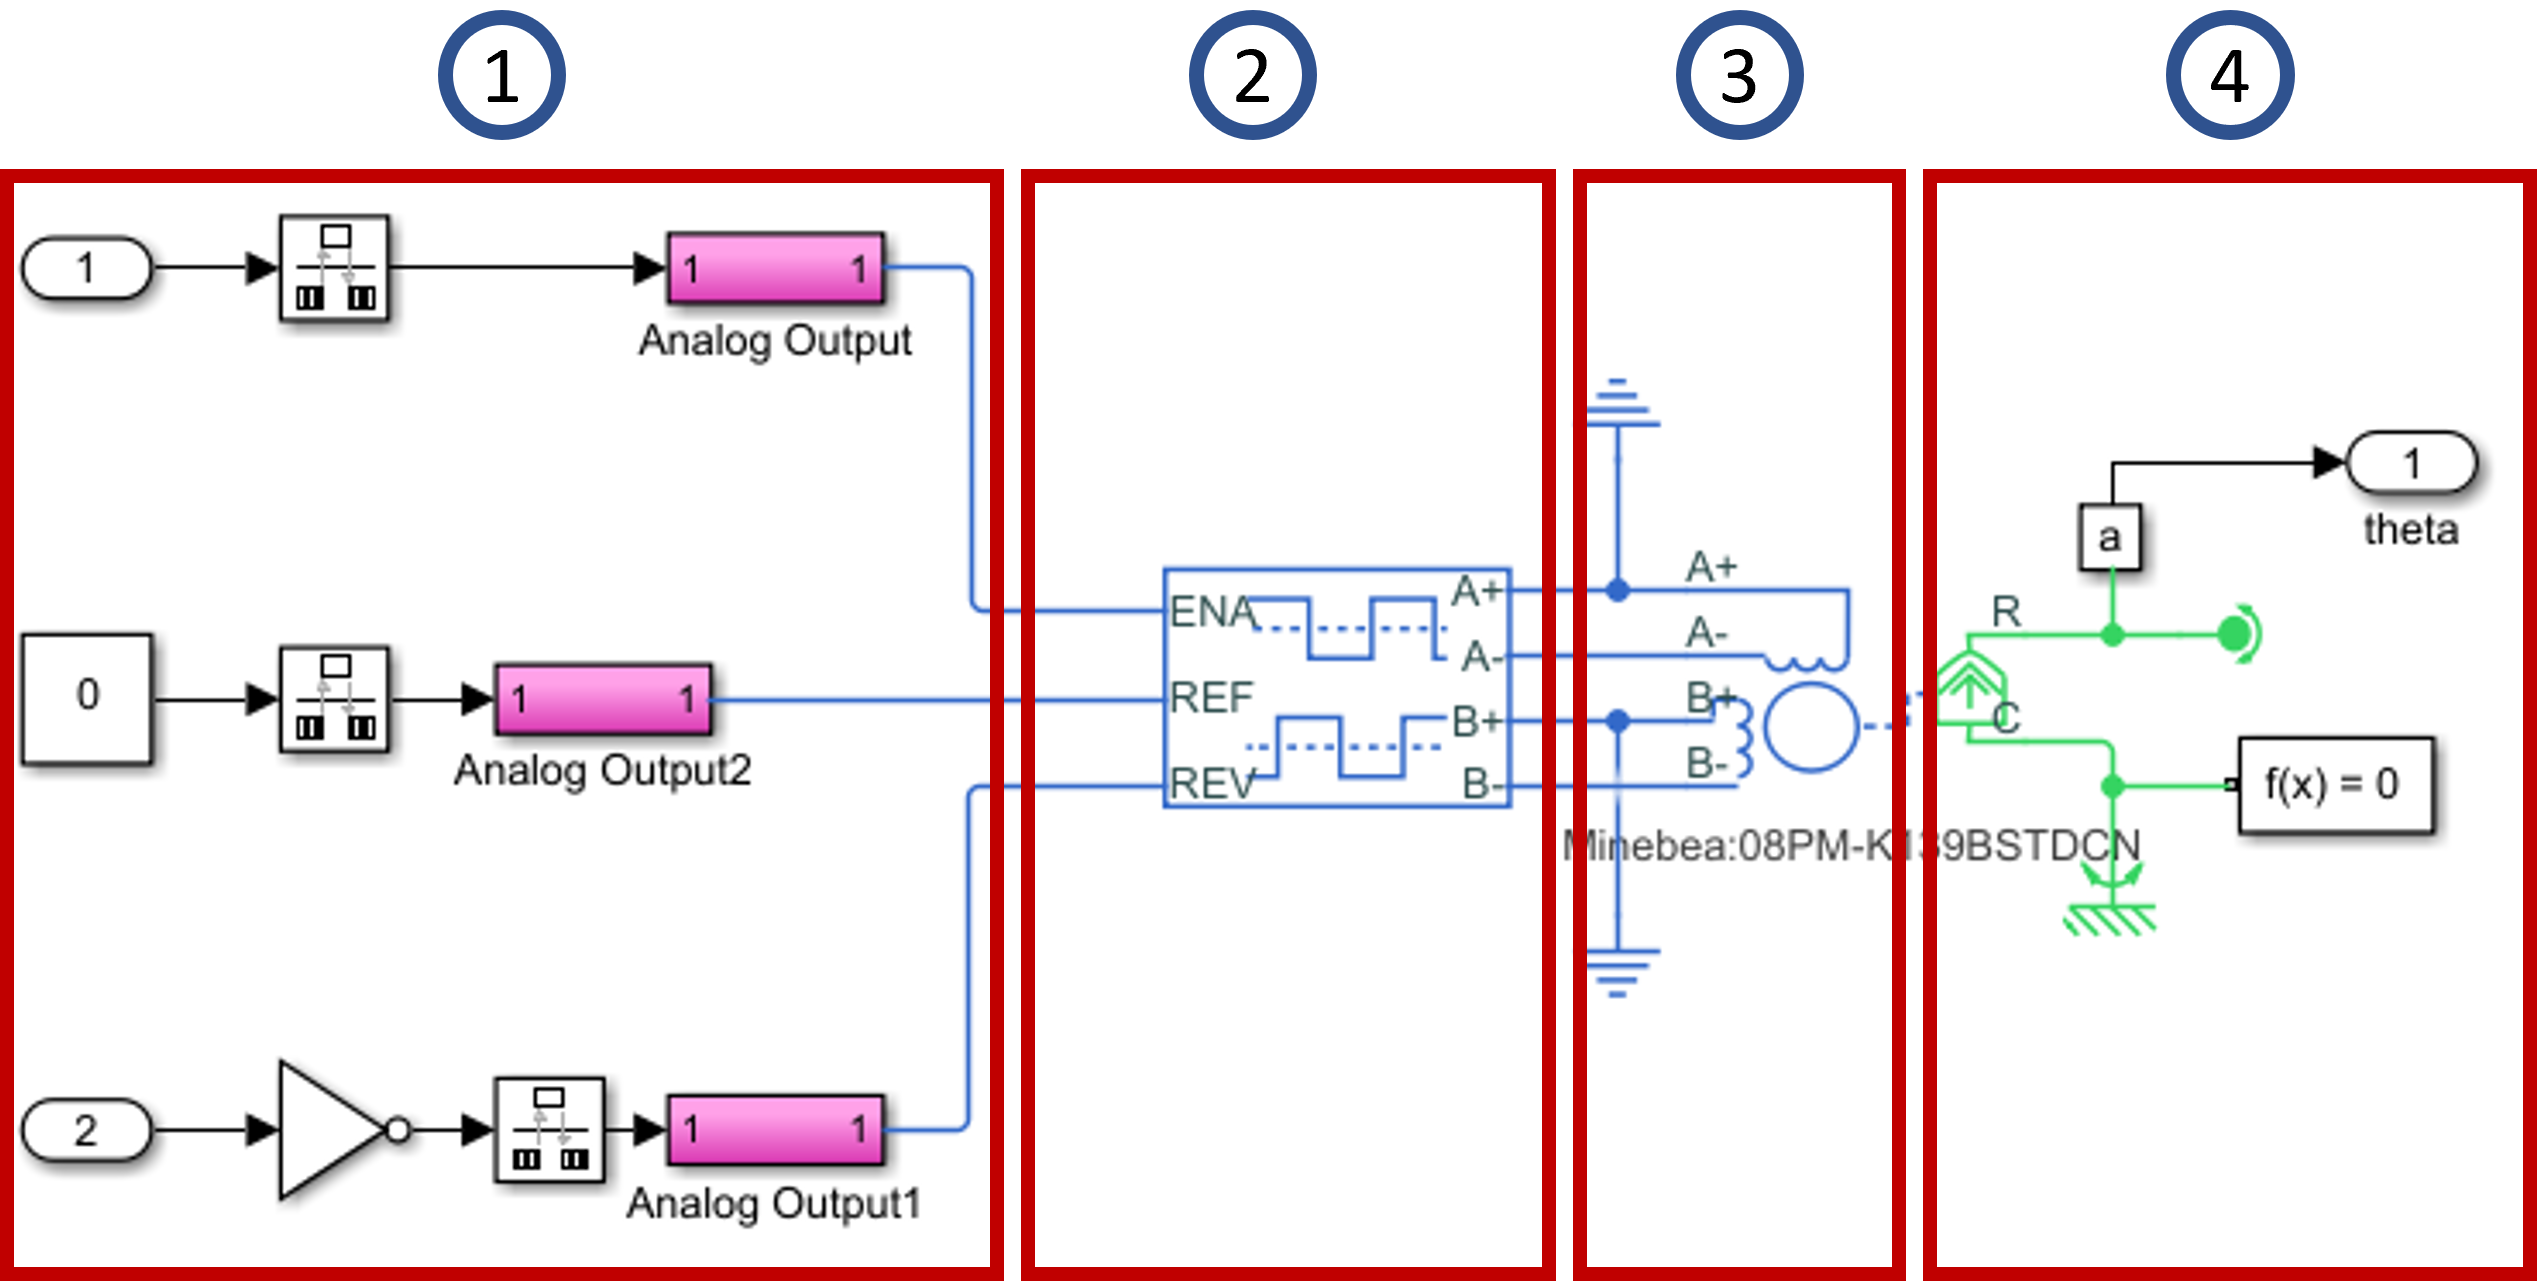
\includegraphics[width=12cm]{Pictures/SysEDriveT.png}
    \caption[Simulink Model of the electronic drive train]{Simulink Model of the electronic drive train; 1 - Input processing, 2 - Motor Controller, 3 - Motor, 4 - Output processing}
    \label{SysEDriveT}
    \end{center}
\end{figure}

It features four sections, first the step and direction signal from Simulink are converted to signal that are compatible with the Simscape system. Second the motor controller is modeled. The third block represents the BLDC motor. However in this case a Stepper motor block was used in order to model the stepwise control of the motor. In the last block of the model the output signal of the motor (angle $\Theta$) is converted back to a numeric Simulink signal.

\subsubsection{Test Bench}

In order to test both hardware and software in an realistic environment the system was assembled in a "Test Bench" configuration. This means, that the inputs into the system can be tightly controlled and every output can be observed. For this reason, the encoder was not connected to the system during this test. It was replaced by another micro controller, which simulated the signal of the encoder. This way, the amount of encoder steps could be precisely determined.
The outputs of the system were connected to both, the motor and an Oscilloscope. This way both, the motor movement as well as the logical signal of the system could be observed.\\

Because the basic functionality of the system was already tested in previous steps, the test performed on the test bench were focused on system performance. System performance was mainly determined by the floating point division that was needed in order to calculate the desired amount of steps. To optimize the processing time of this calculation, two different methods were tested:\\

For the first method that was tested, the translation factor was calculated beforehand. This way the the predefined translation factor has just to be multiplied with the encoder steps. However, this has the big disadvantage, that it will introduce an cumulating rounding error into the calculation. If this method is later used in the final software version, this rounding error has to be investigated.\\

For the second method the translation factor was not calculated beforehand. Everything the encoder position changes the complete translation calculation is done. The equation to calculate the desired Steps is given by:

\begin{equation}
    Encoder Steps * \frac{ Motor Steps * Motor Transmission * Encoder Transmission * Feed Setting}{Encoder Resulution * Leadscrew Slope} 
\end{equation}

With this calculation method the rounding error of the calculation will not cumulate because the calculation is done every time a new Desired Step value is calculated.


\subsection{Integration Test}
The last step in the testing phase is the integration test. This test determines if the behavior of the fully integrated system is matching the specifications. In case of the Electronic Leadscrew, tow different integration tests were performed. First regular turning was tested, second metric and imperial thread cutting was investigated.

\subsubsection{Turning}
The testing of normal turning operation was performed with brass, aluminum and stainless steel. First the maximum possible feed for each of the metal was investigated. This was done with a 1mm depth of cut.
In the second testing phase the best possible surface quality was investigated. This was done with a depth of cut of 0.05mm. The feed of the lathe was than adjusted in order to create the best possible surface finish.

\subsubsection{Threading}
The testing of metric and imperial thread cutting was performed with aluminum and a hand ground HSS threading tool. The main focus during this testing series was the consistency of the thread pitch. For the imperial test a 3/8" thread with 19 threads per inch was chosen. For the metric test a standard M8x1.25 thread was chosen. Both of these threads are very common and could later be checked with thread gauges.












